%%%%%%%%%%%%%%%%%%%%%%%%%%%%%%%%%%%%%%%%%
% Beamer Presentation
% LaTeX Template
% Version 1.0 (10/11/12)
%
% This template has been downloaded from:
% http://www.LaTeXTemplates.com
%
% License:
% CC BY-NC-SA 3.0 (http://creativecommons.org/licenses/by-nc-sa/3.0/)
%
%%%%%%%%%%%%%%%%%%%%%%%%%%%%%%%%%%%%%%%%%
%----------------------------------------------------------------------------------------
%	PACKAGES AND THEMES
%----------------------------------------------------------------------------------------
% Interessante: 
%https://www.codecogs.com/latex/eqneditor.php?lang=pt-br

\documentclass{beamer}

\usepackage[brazilian]{babel}
\usepackage[utf8]{inputenc}
\usepackage[T1]{fontenc}
\usepackage{colortbl}
\usepackage{mathrsfs}
\usepackage{smartdiagram}
\usepackage{listings}
\usepackage[framed,numbered,autolinebreaks,useliterate]{mcode}
\usepackage{multirow}
\usepackage{amssymb}
\usepackage{mdframed}
\usepackage{listings}
\usepackage{amsmath}
\usepackage[framed,numbered,autolinebreaks,useliterate]{mcode}
\usepackage{cancel}

\mode<presentation> {

% The Beamer class comes with a number of default slide themes
% which change the colors and layouts of slides. Below this is a list
% of all the themes, uncomment each in turn to see what they look like.

%\usetheme{default}
%\usetheme{AnnArbor}
%\usetheme{Antibes}
%\usetheme{Bergen}
%\usetheme{Berkeley}
%\usetheme{Berlin}
%\usetheme{Boadilla}
%\usetheme{CambridgeUS}
%\usetheme{Copenhagen}
%\usetheme{Darmstadt}
%\usetheme{Dresden}
\usetheme{Frankfurt}
%\usetheme{Goettingen}
%\usetheme{Hannover}
%\usetheme{Ilmenau}
%\usetheme{JuanLesPins}
%\usetheme{Luebeck}
%\usetheme{Madrid}
%\usetheme{Malmoe}
%\usetheme{Marburg}
%\usetheme{Montpellier}
%\usetheme{PaloAlto}
%\usetheme{Pittsburgh}
%\usetheme{Rochester}
%\usetheme{Singapore}
%\usetheme{Szeged}
%\usetheme{Warsaw}

% As well as themes, the Beamer class has a number of color themes
% for any slide theme. Uncomment each of these in turn to see how it
% changes the colors of your current slide theme.

%\usecolortheme{albatross}
%\usecolortheme{beaver}
%\usecolortheme{beetle}
%\usecolortheme{crane}
%\usecolortheme{dolphin}
%\usecolortheme{dove}
%\usecolortheme{fly}
%\usecolortheme{lily}
%\usecolortheme{orchid}
%\usecolortheme{rose}
%\usecolortheme{seagull}
%\usecolortheme{seahorse}
%\usecolortheme{whale}
%\usecolortheme{wolverine}

%\setbeamertemplate{footline} % To remove the footer line in all slides uncomment this line
%\setbeamertemplate{footline}[page number] % To replace the footer line in all slides with a simple slide count uncomment this line

%\setbeamertemplate{navigation symbols}{} % To remove the navigation symbols from the bottom of all slides uncomment this line
}

\usepackage{graphicx} % Allows including images
\usepackage{booktabs} % Allows the use of \toprule, \midrule and \bottomrule in tables

\usepackage{animate}
\usepackage{hyperref}
\usepackage{media9}
\usepackage{listings}
\usepackage{amsmath}
\usepackage[framed,numbered,autolinebreaks,useliterate]{mcode}
\usepackage{chronology}
\usepackage{xpatch}
\xpretocmd{\chronology}{\tikzset{>=|}}{}{\failure}
\usepackage{mdframed}
\usepackage{tikz}
\usepackage{makecell}

\usepackage{tikz}
\usetikzlibrary{shapes.geometric}
\usetikzlibrary{shapes,arrows}
\usepackage{array}

%----------------------------------------------------------------------------------------
%	TITLE PAGE
%----------------------------------------------------------------------------------------

\logo
{
    
\includegraphics[width=0.6cm,height=0.6cm,keepaspectratio]{UFJF.jpg}~%
}

\title[Aula 5]{Casos Especiais e Dualidade} 

\author{\scriptsize Professores André L.M. Marcato, Ivo C.da Silva Jr, João A.Passos Filho } % Your name
\institute[UFJF/PPEE]{Universidade Federal de Juiz de Fora \\
	Programa de Pós-Graduação em Engenharia Elétrica \\
	\medskip
	\textit{\href{mailto:andre.marcato@ufjf.edu.br}{andre.marcato@ufjf.edu.br}, \href{mailto:ivo.chaves@ufjf.edu.br}{ivo.junior@ufjf.edu.br}, \href{mailto:joao.passos@ufjf.edu.br}{joao.passos@ufjf.edu.br}}
}

%\date{\small \today} % Date, can be changed to a custom date
\date{\small Primeiro Semestre de 2018} % Date, can be changed to a custom date

\hypersetup{
    colorlinks=true,
    linkcolor=gray,
    filecolor=magenta,      
    urlcolor=cyan,
}

\begin{document}

\begin{frame}
\titlepage % Print the title page as the first slide
\begin{figure}[!htb]
\centering
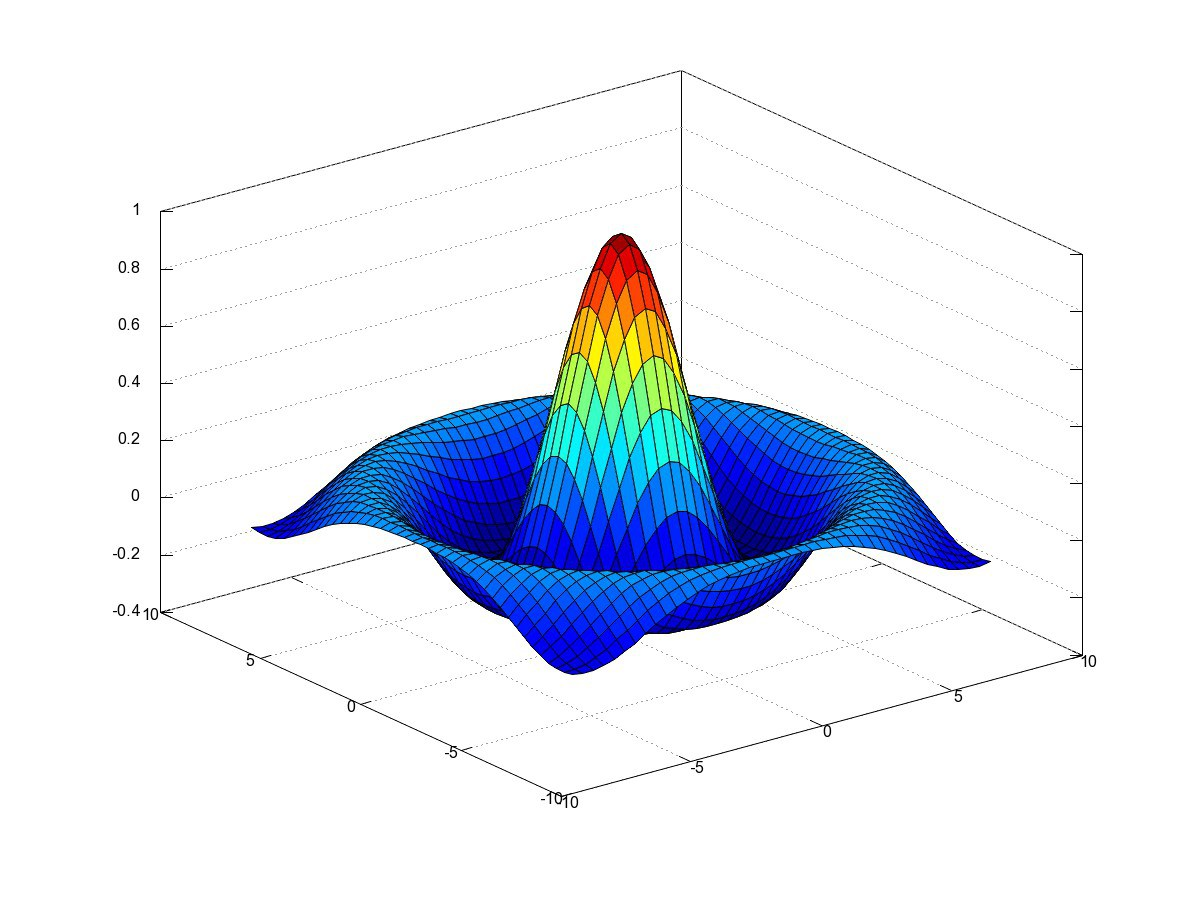
\includegraphics[width=2.6cm, height=1.7cm]{cover.jpg}
%\caption{Ogata - 5a Edicao - Fig. 1.1}
\label{Ogata_1_1}
\end{figure}
\end{frame}

\begin{frame}
\frametitle{Agenda da Apresentação} % Table of contents slide, comment this block out to remove it
\tableofcontents % Throughout your presentation, if you choose to use \section{} and \subsection{} commands, these will automatically be printed on this slide as an overview of your presentation
\end{frame}

%----------------------------------------------------------------------------------------
%	PRESENTATION SLIDES
%----------------------------------------------------------------------------------------

%\section{Método do Big-M}
\subsection{Restrições de Igualdade / Maior ou Igual }
\begin{frame}
	\frametitle{Restrições de Igualdade / Maior ou Igual}
	\begin{columns}
		\begin{column}{0.4\textwidth}
			
\includegraphics[width=5cm,height=4cm]{fique-de-olho.jpg}
		\end{column}
		\begin{column}{0.5\textwidth}
			\begin{itemize}
			\item Soluções Básicas Iniciais devem ser factíveis.
			\item Soluções Factíveis são diretas quando todas as restrições do modelo são da forma $\le$.
			\item Restrições do modelo na forma $\ge$ ou $=$ não levam a obenção direta de soluções iniciais factíveis.
			\end{itemize}
		\end{column}
	\end{columns}
\end{frame}

\begin{frame}
	\frametitle{Exemplo}
	\begin{columns}
		\begin{column}{0.5\textwidth}
			\begin{block}{Encontre uma SBF Inicial para:}
				\centering
				$
					\begin{matrix}
						\scriptstyle \max Z = 3x_1 + 2,5x_2 + 1,2x_3 \\
						\scriptstyle \text{Sujeito à:}\\
						\scriptstyle x_1 -2x_2 + 4x_3 \le 40 \\
						\scriptstyle x_1 +x_2  + 2x_3 \ge 60 \\
						\scriptstyle 2x_1 +3x_2 + x_3 = 15 \\
						\scriptstyle x_1, x_2, x_3 \ge 0 \\
					\end{matrix}
				$
			\end{block}
		\end{column} \pause
		\begin{column}{0.5\textwidth}
			\begin{exampleblock}{Forma Padrão:}
				\centering
				$
					\begin{matrix}
						\scriptstyle \max Z = 3x_1 + 2,5x_2 + 1,2x_3 \\
						\scriptstyle \text{Sujeito à:}\\
						\scriptstyle x_1 -2x_2 + 4x_3 {\color{red}+x_4 =} 40 \\
						\scriptstyle x_1 +x_2  + 2x_3 {\color{red}-x_5=} 60 \\
						\scriptstyle 2x_1 +3x_2 + x_3 = 15 \\
						\scriptstyle x_1, x_2, x_3{\color{red},x_4,x_5} \ge 0 \\
					\end{matrix}
				$
			\end{exampleblock}
		\end{column} \pause
	\end{columns}

	\vspace{0.8cm}

	\begin{columns}
		\begin{column}{0.5\textwidth}
			$
				\begin{matrix}
					VNB \left\{
								\begin{matrix}
												x_1 = 0 \\
												x_2 = 0 \\
												x_3 = 0 \\
								\end{matrix} 
						\right. &
					VB \left\{
								\begin{matrix}
												x_4 = 40 \\
												{\color{red} x_5 = -60} \\
								\end{matrix} 
						\right. \\		
					 &  \\				
				\end{matrix}
			$
			$ {\color{red}0 + 0 + 0 = 15}  $
			
		\end{column} \pause
		\begin{column}{0.5\textwidth}
			\centering
			
\includegraphics[width=3cm,height=3cm]{houston.jpg}
		\end{column}
	\end{columns}
\end{frame}

\begin{frame}
	\centering
	
\includegraphics[width=10cm,height=3cm]{Pergunta_Final.png}
	\begin{columns}
		\begin{column}{0.33\textwidth}
			\only<1>
			{
				\begin{mdframed}[backgroundcolor=green!80]
					\centering
					Método das Penalidades (BIG-M)
				\end{mdframed}
			}		
			\only<2>
			{
				\begin{mdframed}[backgroundcolor=red!80]
					\centering
					Método das Penalidades (BIG-M)
				\end{mdframed}
			}		
		\end{column}
		\begin{column}{0.33\textwidth}
			\centering
			
\includegraphics[width=4cm,height=4cm]{twoways.jpg}
		\end{column}
		\hspace{0.2cm}
		\begin{column}{0.33\textwidth}
			\begin{mdframed}[backgroundcolor=green!80]
				\centering
				Método das Duas Fases
			\end{mdframed}		
		\end{column}
	\end{columns}
\end{frame}

\begin{frame}
	\frametitle{O Método do Big M}
	\begin{itemize}
	\item[] {Este método consiste em acrescentar na FOB do problema original (\textbf{forma padrão}) variáveis artificiais - $\mathbf{\color{red}a}$ - com penalidades - $\mathbf{\color{red}M}$:} \pause
		\begin{itemize}
		\item {Negativos Muito Grandes - Problemas de Maximização} 
			\begin{mdframed}[backgroundcolor=green!80,rightmargin=4.8cm]
			$
			\max Z = 2x_1 + 3x_2 \color{red}\boxed{-Ma}
			$
			\end{mdframed} \pause
		\item {Positivos muito grandes - Problemas de Minimização}
			\begin{mdframed}[backgroundcolor=green!80,rightmargin=4.8cm]
			$
			\max Z = 2x_1 + 3x_2 \color{red}\boxed{+Ma}
			$
			\end{mdframed} \pause
		\end{itemize}
	\end{itemize}
	\begin{columns}
		\begin{column}{0.3\textwidth}
			\centering
			
\includegraphics[width=3cm,height=3cm]{importante.jpg} 
		\end{column}
		\begin{column}{0.7\textwidth}
			Na solução final os valores das variáveis artificiais devem ser nulos (VNB).		
		\end{column}
	\end{columns}
\end{frame}

\subsection{Exemplo}

\begin{frame}
	\frametitle{Exemplo}
	\begin{columns}
		\begin{column}{5cm}
			\begin{block}{Resolver o seguinte PPL}
				\centering
				$
					\begin{matrix}
						\max 2x_1+3x_2 \\
						\text{Sujeito a} \\
						-2x_1+3x_2 \le 6 \\
						x_1 + 2x_2 \ge 8 \\
						x_1 + x_2 = 6 \\
						x_1, x_2 \ge 0 \\
					\end{matrix}
				$
			\end{block} \pause
		\end{column}
		\begin{column}{5cm}
			\begin{exampleblock}{Forma Padrão}
				\centering
				$
					\begin{matrix}
						\max 2x_1+3x_2 \\
						\text{Sujeito a} \\
						-2x_1+3x_2 {\color{red}+x_3=} 6 \\
						x_1 + 2x_2 {\color{red}-x_4=} 8 \\
						x_1 + x_2 = 6 \\
						x_1, x_2{\color{red},x_3,x_4} \ge 0 \\
					\end{matrix}
				$
			\end{exampleblock} \pause
		\end{column}
	\end{columns}
	\vspace{0.5cm}
	\begin{columns}
		\begin{column}{4cm}
			$
				\begin{matrix}
					VNB \left\{ 
								\begin{matrix}
												x_1 = 0 \\
												x_2 = 0 \\
								\end{matrix}
						\right. &
					VB \left\{
								\begin{matrix}
									x_3 = 6 \\
									x_4 = -8 \\
								\end{matrix}
						\right. \\ 
					& \\
				\end{matrix}
			$
			$ Z = 0 $ \pause
		\end{column}
		\begin{column}{5cm}
			\scriptsize
			\begin{itemize}
			\item[] \underline{Problemas:}
			\item $x_4 = 8$, deveria ser maior que zero.
			\item $x_1+x_2=6$, igualdade não satisfeita.
			\item Não possui solução inicial trivial.
			\end{itemize}
		\end{column}
	\end{columns}
\end{frame}


\begin{frame}
	\frametitle{Exemplo}
	\begin{columns}
		\begin{column}{5cm}
			\begin{block}{Resolver o seguinte PPL}
				\centering
				$
					\begin{matrix}
						\max 2x_1+3x_2 \\
						\text{Sujeito a} \\
						-2x_1+3x_2 \le 6 \\
						x_1 + 2x_2 \ge 8 \\
						x_1 + x_2 = 6 \\
						x_1, x_2 \ge 0 \\
					\end{matrix}
				$
			\end{block}
		\end{column}
		\begin{column}{5cm}
			\begin{exampleblock}{Forma Padrão}
				\centering
				$
					\begin{matrix}
						\max 2x_1+3x_2 \\
						\text{Sujeito a} \\
						-2x_1+3x_2 {\color{red}+x_3=} 6 \\
						x_1 + 2x_2 {\color{red}-x_4=} 8 \\
						x_1 + x_2 = 6 \\
						x_1, x_2{\color{red},x_3,x_4} \ge 0 \\
					\end{matrix}
				$
			\end{exampleblock}
		\end{column}
	\end{columns}
	\only<1>
	{
		\begin{alertblock}{\centering Inserção das Variáveis Artificiais e das Penalidades}
					\centering
					$
						\begin{matrix}
							\max Z - 2x_1-3x_2  &                                       &                   & \cellcolor{green!70}{\color{red}+Mx_5} & \cellcolor{green!70}{\color{red}+ Mx_6}  & =0 \\
							\text{Sujeito a} \\
							-2x_1+3x_2          & \cellcolor{green!70}{\color{red}+x_3} &                   &                                        &                                          & =6 \\
							x_1 + 2x_2          &                                       & {\color{red}-x_4} & \cellcolor{green!70}{\color{red}+x_5}  &                                          & =8 \\
							x_1 + x_2           &                                       &                   &                                        & \cellcolor{green!70}{\color{red}+x_6}    & =6 \\
							x_1, x_2{\color{red},x_3,x_4,x_5,x_6} \ge 0 \\
						\end{matrix}
					$
		\end{alertblock}
	}
	\only<2-3>
	{
			\vspace{0.5cm}
			\centering
			$
				\begin{matrix}
					VNB \left\{ 
								\begin{matrix}
												x_1 = 0 \\
												x_2 = 0 \\
												x_4 = 0 \\
								\end{matrix}
						\right. &
					VB \left\{
								\begin{matrix}
									x_3 = 6 \\
									x_5 = 8 \\
									x_6 = 6 \\
								\end{matrix}
						\right. 
					& Z = 0\\
				\end{matrix}
			$
	}	
	\only<3>
	{
		\begin{columns}
			\begin{column}{1cm}
				
\includegraphics[width=2cm,height=1.3cm]{atencao.jpg}
			\end{column}
			\begin{column}{9cm}
				\color{red}\Large A FOB deve conter somente VNB !
			\end{column}
		\end{columns}
	}
\end{frame}

\begin{frame}
	\frametitle{Exemplo}
	\only<1-2>
	{
		\begin{alertblock}{\centering Inserção das Variáveis Artificiais e das Penalidades}
					\centering
					$
						\begin{matrix}
							\max Z - 2x_1-3x_2  &                                       &                   & \cellcolor{green!70}{\color{red}+Mx_5} & \cellcolor{green!70}{\color{red}+ Mx_6}  & =0 \\
							\text{Sujeito a} \\
							-2x_1+3x_2          & \cellcolor{green!70}{\color{red}+x_3} &                   &                                        &                                          & =6 \\
							x_1 + 2x_2          &                                       & {\color{red}-x_4} & \cellcolor{green!70}{\color{red}+x_5}  &                                          & =8 \\
							x_1 + x_2           &                                       &                   &                                        & \cellcolor{green!70}{\color{red}+x_6}    & =6 \\
							x_1, x_2{\color{red},x_3,x_4,x_5,x_6} \ge 0 \\
						\end{matrix}
					$
		\end{alertblock}
	}	
	\only<3>
	{
		\begin{alertblock}{\centering Inserção das Variáveis Artificiais e das Penalidades}
					\centering
					$
						\begin{matrix}
							\scriptstyle \max Z - 2x_1-3x_2  &                                                    &                               & \scriptstyle \cellcolor{green!70}{\color{red}+M(8-x_1-2x_2+x_4)} & \scriptstyle \cellcolor{green!70}{\color{red}+ M(6-x_1-x_2)}  & \scriptstyle =0 \\
							\scriptstyle \text{Sujeito a} \\
							\scriptstyle -2x_1+3x_2          & \scriptstyle \cellcolor{green!70}{\color{red}+x_3} &                               &                                                                  &                                                               & \scriptstyle =6 \\
							\scriptstyle x_1 + 2x_2          &                                                    & \scriptstyle{\color{red}-x_4} & \scriptstyle \cellcolor{green!70}{\color{red}+x_5}               &                                                               & \scriptstyle =8 \\
							\scriptstyle x_1 + x_2           &                                                    &                               &                                                                  & \scriptstyle \cellcolor{green!70}{\color{red}+x_6}            & \scriptstyle =6 \\
							\scriptstyle x_1, x_2{\color{red},x_3,x_4,x_5,x_6} \ge 0 \\
						\end{matrix}
					$
		\end{alertblock}
	}
	\only<4-5>
	{
		\begin{alertblock}{\centering Inserção das Variáveis Artificiais e das Penalidades}

			$ \max Z + (-2-2M) x_1 + (-3-3M) x_2 + Mx_4 + 14M = 0 $ \\
			{\textbf{Sujeito à}}: \\
			$
				\begin{matrix}
					-2x_1+3x_2+   & {\color{red}x_3} &                  &  					& = 6 \\
					x_1+2x_2-x_4  &				     & \color{red}+x_5  &  					& = 8 \\
					x_1+x_2		  &			         &				   & \color{red}+x_6 	& = 6 \\
					x_1, x_2, x_3,x_4,x_5,x_6 \ge 0  \\
				\end{matrix}
			$
		\end{alertblock}
	}		
	
	\only<2-3>
	{
		\begin{itemize}
		\item[] $x_5 = 8-x_1-2x_2+x_4$
		\item[] $x_6 = 6-x_1-x_2$
		\end{itemize}
	
	}
	\only<4-5>
	{
			\vspace{0.5cm}
			\centering
			$
				\begin{matrix}
					VNB \left\{ 
								\begin{matrix}
												x_1 = 0 \\
												x_2 = 0 \\
												x_4 = 0 \\
								\end{matrix}
						\right. &
					VB \left\{
								\begin{matrix}
									x_3 = 6 \\
									x_5 = 8 \\
									x_6 = 6 \\
								\end{matrix}
						\right. 
					& Z = -14M\\
				\end{matrix}
			$
	}
	\only<5>
	{
		\begin{columns}
			\begin{column}{1cm}
				
\includegraphics[width=2cm,height=2cm]{OK.png}
			\end{column}
			\begin{column}{9cm}
				\color{red}\Large A FOB contém somente VNB ! \\
				\color{black}\normalsize \underline{Em geral}, atribui-se a M um valor 20 vezes superior ao maior coeficiente da FOB original.
			\end{column}
		\end{columns}
	}	
\end{frame}

\begin{frame}
	\only<1-5>
	{
		\frametitle{Exemplo - Busca Tableau - \color{cyan} $1^a$ Iteração}
	}
	\only<6-9>
	{
		\frametitle{Exemplo - Busca Tableau - \color{cyan} $2^a$ Iteração}
	}
	\only<10-13>
	{
		\frametitle{Exemplo - Busca Tableau - \color{cyan} $3^a$ Iteração}
	}
	\only<14->
	{
		\frametitle{Exemplo - Busca Tableau - \color{cyan} $4^a$ Iteração}
	}

	\only<1>
	{
		\begin{table}		
			\begin{tabular}{c c c c c c c c c c c c}
				\cline{1-8} 
				\cellcolor{blue!100} \color{white} \scriptsize Base 
				&\cellcolor{blue!100} \color{white} \scriptsize Z 
				&\cellcolor{blue!100} \color{white} $\scriptstyle X_1$ 
				&\cellcolor{blue!100} \color{white} $\scriptstyle X_2$ 
				&\cellcolor{blue!100} \color{red}   $\scriptstyle X_3$ 
				&\cellcolor{blue!100} \color{white} $\scriptstyle X_4$ 
				&\cellcolor{blue!100} \color{red}   $\scriptstyle X_5$ 
				&\cellcolor{blue!100} \color{red}   $\scriptstyle X_6$ 
				&\cellcolor{blue!100} \color{white} \scriptsize b
				&
				&
				& \\
				\cellcolor{blue!100} \color{red} $\scriptstyle X_3$
				& \cellcolor{yellow!50} $\scriptstyle 0$
				& \cellcolor{yellow!50} $\scriptstyle -2$
				& \cellcolor{yellow!50} $\scriptstyle +3$
				& \cellcolor{yellow!50} $\scriptstyle +1$
				& \cellcolor{yellow!50} $\scriptstyle 0$
				& \cellcolor{yellow!50} $\scriptstyle 0$
				& \cellcolor{yellow!50} $\scriptstyle 0$
				& \cellcolor{yellow!50} $\scriptstyle +6$ \\
			    \cellcolor{blue!100} \color{red} $\scriptstyle X_5$
				& \cellcolor{yellow!50} $\scriptstyle 0$
				& \cellcolor{yellow!50} $\scriptstyle +1$
				& \cellcolor{yellow!50} $\scriptstyle +2$
				& \cellcolor{yellow!50} $\scriptstyle 0$			
				& \cellcolor{yellow!50} $\scriptstyle -1$
				& \cellcolor{yellow!50} $\scriptstyle +1$
				& \cellcolor{yellow!50} $\scriptstyle 0$ 
				& \cellcolor{yellow!50} $\scriptstyle +8$ \\
				\cellcolor{blue!100} \color{red} $\scriptstyle X_6$
				& \cellcolor{yellow!50} $\scriptstyle 0$
				& \cellcolor{yellow!50} $\scriptstyle +1$
				& \cellcolor{yellow!50} $\scriptstyle +1$
				& \cellcolor{yellow!50} $\scriptstyle 0$
				& \cellcolor{yellow!50} $\scriptstyle 0$
				& \cellcolor{yellow!50} $\scriptstyle 0$
				& \cellcolor{yellow!50} $\scriptstyle +1$
				& \cellcolor{yellow!50} $\scriptstyle +6$ \\
				\cellcolor{blue!100} \color{white} $\scriptstyle Z$
				& \cellcolor{yellow!50} $\scriptstyle +1$
				& \cellcolor{yellow!50} $\scriptstyle (-2-2M)$
				& \cellcolor{yellow!50} $\scriptstyle (-3-3M)$
				& \cellcolor{yellow!50} $\scriptstyle 0$
				& \cellcolor{yellow!50} $\scriptstyle M$
				& \cellcolor{yellow!50} $\scriptstyle 0$
				& \cellcolor{yellow!50} $\scriptstyle 0$ 
				& \cellcolor{yellow!50} $\scriptstyle -14M$  \\
			\end{tabular}
		\end{table}			
	}
	\only<2>
	{
		\begin{table}		
			\begin{tabular}{c c c c c c c c c c c c}
				\cline{1-8} 
				\cellcolor{blue!100} \color{white} \scriptsize Base 
				&\cellcolor{blue!100} \color{white} \scriptsize Z 
				&\cellcolor{blue!100} \color{white} $\scriptstyle X_1$ 
				&\cellcolor{blue!100} \color{white} $\scriptstyle X_2$ 
				&\cellcolor{blue!100} \color{red}   $\scriptstyle X_3$ 
				&\cellcolor{blue!100} \color{white} $\scriptstyle X_4$ 
				&\cellcolor{blue!100} \color{red}   $\scriptstyle X_5$ 
				&\cellcolor{blue!100} \color{red}   $\scriptstyle X_6$ 
				&\cellcolor{blue!100} \color{white} \scriptsize b
				&
				&
				& \\
				\cellcolor{blue!100} \color{red} $\scriptstyle X_3$
				& \cellcolor{yellow!50} $\scriptstyle 0$
				& \cellcolor{yellow!50} $\scriptstyle -2$
				& \cellcolor{yellow!50} $\scriptstyle +3$
				& \cellcolor{yellow!50} $\scriptstyle +1$
				& \cellcolor{yellow!50} $\scriptstyle 0$
				& \cellcolor{yellow!50} $\scriptstyle 0$
				& \cellcolor{yellow!50} $\scriptstyle 0$
				& \cellcolor{yellow!50} $\scriptstyle +6$ \\
			    \cellcolor{blue!100} \color{red} $\scriptstyle X_5$
				& \cellcolor{yellow!50} $\scriptstyle 0$
				& \cellcolor{yellow!50} $\scriptstyle +1$
				& \cellcolor{yellow!50} $\scriptstyle +2$
				& \cellcolor{yellow!50} $\scriptstyle 0$			
				& \cellcolor{yellow!50} $\scriptstyle -1$
				& \cellcolor{yellow!50} $\scriptstyle +1$
				& \cellcolor{yellow!50} $\scriptstyle 0$ 
				& \cellcolor{yellow!50} $\scriptstyle +8$ \\
				\cellcolor{blue!100} \color{red} $\scriptstyle X_6$
				& \cellcolor{yellow!50} $\scriptstyle 0$
				& \cellcolor{yellow!50} $\scriptstyle +1$
				& \cellcolor{yellow!50} $\scriptstyle +1$
				& \cellcolor{yellow!50} $\scriptstyle 0$
				& \cellcolor{yellow!50} $\scriptstyle 0$
				& \cellcolor{yellow!50} $\scriptstyle 0$
				& \cellcolor{yellow!50} $\scriptstyle +1$
				& \cellcolor{yellow!50} $\scriptstyle +6$ \\
				\cellcolor{blue!100} \color{white} $\scriptstyle Z$
				& \cellcolor{yellow!50} $\scriptstyle +1$
				& \cellcolor{yellow!50} $\scriptstyle -122$
				& \cellcolor{yellow!50} $\scriptstyle -183$
				& \cellcolor{yellow!50} $\scriptstyle 0$
				& \cellcolor{yellow!50} $\scriptstyle +60$
				& \cellcolor{yellow!50} $\scriptstyle 0$
				& \cellcolor{yellow!50} $\scriptstyle 0$ 
				& \cellcolor{yellow!50} $\scriptstyle -840$  \\
			\end{tabular}
		\end{table}			
	}
	\only<3>
	{
		\begin{table}		
			\begin{tabular}{c c c c c c c c c c c c}
				\cline{1-8} 
				\cellcolor{blue!100} \color{white} \scriptsize Base 
				&\cellcolor{blue!100} \color{white} \scriptsize Z 
				&\cellcolor{blue!100} \color{white} $\scriptstyle X_1$ 
				&\cellcolor{blue!100} \color{white} $\scriptstyle X_2$ 
				&\cellcolor{blue!100} \color{red}   $\scriptstyle X_3$ 
				&\cellcolor{blue!100} \color{white} $\scriptstyle X_4$ 
				&\cellcolor{blue!100} \color{red}   $\scriptstyle X_5$ 
				&\cellcolor{blue!100} \color{red}   $\scriptstyle X_6$ 
				&\cellcolor{blue!100} \color{white} \scriptsize b
				&
				&
				& \\
				\cellcolor{blue!100} \color{red} $\scriptstyle X_3$
				& \cellcolor{yellow!50} $\scriptstyle 0$
				& \cellcolor{yellow!50} $\scriptstyle -2$
				& \cellcolor{gray!50} $\scriptstyle +3$
				& \cellcolor{yellow!50} $\scriptstyle +1$
				& \cellcolor{yellow!50} $\scriptstyle 0$
				& \cellcolor{yellow!50} $\scriptstyle 0$
				& \cellcolor{yellow!50} $\scriptstyle 0$
				& \cellcolor{yellow!50} $\scriptstyle +6$ \\
			    \cellcolor{blue!100} \color{red} $\scriptstyle X_5$
				& \cellcolor{yellow!50} $\scriptstyle 0$
				& \cellcolor{yellow!50} $\scriptstyle +1$
				& \cellcolor{gray!50} $\scriptstyle +2$
				& \cellcolor{yellow!50} $\scriptstyle 0$			
				& \cellcolor{yellow!50} $\scriptstyle -1$
				& \cellcolor{yellow!50} $\scriptstyle +1$
				& \cellcolor{yellow!50} $\scriptstyle 0$ 
				& \cellcolor{yellow!50} $\scriptstyle +8$ \\
				\cellcolor{blue!100} \color{red} $\scriptstyle X_6$
				& \cellcolor{yellow!50} $\scriptstyle 0$
				& \cellcolor{yellow!50} $\scriptstyle +1$
				& \cellcolor{gray!50} $\scriptstyle +1$
				& \cellcolor{yellow!50} $\scriptstyle 0$
				& \cellcolor{yellow!50} $\scriptstyle 0$
				& \cellcolor{yellow!50} $\scriptstyle 0$
				& \cellcolor{yellow!50} $\scriptstyle +1$
				& \cellcolor{yellow!50} $\scriptstyle +6$ \\
				\cellcolor{blue!100} \color{white} $\scriptstyle Z$
				& \cellcolor{yellow!50} $\scriptstyle +1$
				& \cellcolor{yellow!50} $\scriptstyle -122$
				& \cellcolor{gray!50} $\scriptstyle -183$
				& \cellcolor{yellow!50} $\scriptstyle 0$
				& \cellcolor{yellow!50} $\scriptstyle +60$
				& \cellcolor{yellow!50} $\scriptstyle 0$
				& \cellcolor{yellow!50} $\scriptstyle 0$ 
				& \cellcolor{yellow!50} $\scriptstyle -840$  \\
				& & & 
\includegraphics[width=0.3cm,height=0.3cm]{setacima.jpg} \\
				& & & \scriptsize Entra\\ 
			\end{tabular}
		\end{table}			
	}
	\only<4>
	{
		\begin{table}		
			\begin{tabular}{c c c c c c c c c c c c}
				\cline{1-8} 
				\cellcolor{blue!100} \color{white} \scriptsize Base 
				&\cellcolor{blue!100} \color{white} \scriptsize Z 
				&\cellcolor{blue!100} \color{white} $\scriptstyle X_1$ 
				&\cellcolor{blue!100} \color{white} $\scriptstyle X_2$ 
				&\cellcolor{blue!100} \color{red}   $\scriptstyle X_3$ 
				&\cellcolor{blue!100} \color{white} $\scriptstyle X_4$ 
				&\cellcolor{blue!100} \color{red}   $\scriptstyle X_5$ 
				&\cellcolor{blue!100} \color{red}   $\scriptstyle X_6$ 
				&\cellcolor{blue!100} \color{white} \scriptsize b
				&
				&
				& \\
				\cellcolor{blue!100} \color{red} $\scriptstyle X_3$
				& \cellcolor{yellow!50} $\scriptstyle 0$
				& \cellcolor{yellow!50} $\scriptstyle -2$
				& \cellcolor{gray!50} $\scriptstyle +3$
				& \cellcolor{yellow!50} $\scriptstyle +1$
				& \cellcolor{yellow!50} $\scriptstyle 0$
				& \cellcolor{yellow!50} $\scriptstyle 0$
				& \cellcolor{yellow!50} $\scriptstyle 0$
				& \cellcolor{gray!50} $\scriptstyle +6$
				& $\scriptstyle \frac{+6}{+3}=+2$ & 
\includegraphics[width=0.3cm,height=0.3cm]{setaesquerda.jpg} \\
			    \cellcolor{blue!100} \color{red} $\scriptstyle X_5$
				& \cellcolor{yellow!50} $\scriptstyle 0$
				& \cellcolor{yellow!50} $\scriptstyle +1$
				& \cellcolor{gray!50} $\scriptstyle +2$
				& \cellcolor{yellow!50} $\scriptstyle 0$			
				& \cellcolor{yellow!50} $\scriptstyle -1$
				& \cellcolor{yellow!50} $\scriptstyle +1$
				& \cellcolor{yellow!50} $\scriptstyle 0$ 
				& \cellcolor{gray!50} $\scriptstyle +8$ 
				& $\scriptstyle \frac{+8}{+2}=+4$ & 
\includegraphics[width=0.3cm,height=0.3cm]{setaesquerda.jpg} \\
				\cellcolor{blue!100} \color{red} $\scriptstyle X_6$
				& \cellcolor{yellow!50} $\scriptstyle 0$
				& \cellcolor{yellow!50} $\scriptstyle +1$
				& \cellcolor{gray!50} $\scriptstyle +1$
				& \cellcolor{yellow!50} $\scriptstyle 0$
				& \cellcolor{yellow!50} $\scriptstyle 0$
				& \cellcolor{yellow!50} $\scriptstyle 0$
				& \cellcolor{yellow!50} $\scriptstyle +1$
				& \cellcolor{gray!50} $\scriptstyle +6$ 
				& $\scriptstyle \frac{+6}{+1}=+6$ & 
\includegraphics[width=0.3cm,height=0.3cm]{setaesquerda.jpg}\\
				\cellcolor{blue!100} \color{white} $\scriptstyle Z$
				& \cellcolor{yellow!50} $\scriptstyle +1$
				& \cellcolor{yellow!50} $\scriptstyle -122$
				& \cellcolor{gray!50} $\scriptstyle -183$
				& \cellcolor{yellow!50} $\scriptstyle 0$
				& \cellcolor{yellow!50} $\scriptstyle +60$
				& \cellcolor{yellow!50} $\scriptstyle 0$
				& \cellcolor{yellow!50} $\scriptstyle 0$ 
				& \cellcolor{gray!50} $\scriptstyle -840$  \\
				& & & 
\includegraphics[width=0.3cm,height=0.3cm]{setacima.jpg} \\
				& & & \scriptsize Entra \\ 
			\end{tabular}
		\end{table}			
	}
	\only<5>
	{
		\begin{table}		
			\begin{tabular}{c c c c c c c c c c c c}
				\cline{1-8} 
				\cellcolor{blue!100} \color{white} \scriptsize Base 
				&\cellcolor{blue!100} \color{white} \scriptsize Z 
				&\cellcolor{blue!100} \color{white} $\scriptstyle X_1$ 
				&\cellcolor{blue!100} \color{white} $\scriptstyle X_2$ 
				&\cellcolor{blue!100} \color{red}   $\scriptstyle X_3$ 
				&\cellcolor{blue!100} \color{white} $\scriptstyle X_4$ 
				&\cellcolor{blue!100} \color{red}   $\scriptstyle X_5$ 
				&\cellcolor{blue!100} \color{red}   $\scriptstyle X_6$ 
				&\cellcolor{blue!100} \color{white} \scriptsize b
				&
				&
				& \\
				\cellcolor{blue!100} \color{red} $\scriptstyle X_3$
				& \cellcolor{gray!50} $\scriptstyle 0$
				& \cellcolor{gray!50} $\scriptstyle -2$
				& \cellcolor{red!50} $\scriptstyle +3$
				& \cellcolor{gray!50} $\scriptstyle +1$
				& \cellcolor{gray!50} $\scriptstyle 0$
				& \cellcolor{gray!50} $\scriptstyle 0$
				& \cellcolor{gray!50} $\scriptstyle 0$
				& \cellcolor{gray!50} $\scriptstyle +6$
				& $\scriptstyle \frac{+6}{+3}=+2$ &
				
\includegraphics[width=0.3cm,height=0.3cm]{setaesquerda.jpg} \scriptsize Sai \\
			    \cellcolor{blue!100} \color{red} $\scriptstyle X_5$
				& \cellcolor{yellow!50} $\scriptstyle 0$
				& \cellcolor{yellow!50} $\scriptstyle +1$
				& \cellcolor{gray!50} $\scriptstyle +2$
				& \cellcolor{yellow!50} $\scriptstyle 0$			
				& \cellcolor{yellow!50} $\scriptstyle -1$
				& \cellcolor{yellow!50} $\scriptstyle +1$
				& \cellcolor{yellow!50} $\scriptstyle 0$ 
				& \cellcolor{gray!50} $\scriptstyle +8$  \\
				\cellcolor{blue!100} \color{red} $\scriptstyle X_6$
				& \cellcolor{yellow!50} $\scriptstyle 0$
				& \cellcolor{yellow!50} $\scriptstyle +1$
				& \cellcolor{gray!50} $\scriptstyle +1$
				& \cellcolor{yellow!50} $\scriptstyle 0$
				& \cellcolor{yellow!50} $\scriptstyle 0$
				& \cellcolor{yellow!50} $\scriptstyle 0$
				& \cellcolor{yellow!50} $\scriptstyle +1$
				& \cellcolor{gray!50} $\scriptstyle +6$ \\
				\cellcolor{blue!100} \color{white} $\scriptstyle Z$
				& \cellcolor{yellow!50} $\scriptstyle +1$
				& \cellcolor{yellow!50} $\scriptstyle -122$
				& \cellcolor{gray!50} $\scriptstyle -183$
				& \cellcolor{yellow!50} $\scriptstyle 0$
				& \cellcolor{yellow!50} $\scriptstyle +60$
				& \cellcolor{yellow!50} $\scriptstyle 0$
				& \cellcolor{yellow!50} $\scriptstyle 0$ 
				& \cellcolor{gray!50} $\scriptstyle -840$  \\
				& & & 
\includegraphics[width=0.3cm,height=0.3cm]{setacima.jpg} \\
				& & & \scriptsize Entra \\ 
			\end{tabular}
		\end{table}			
	}
	\only<6>
	{
		\begin{table}		
			\begin{tabular}{c c c c c c c c c c c c}
				\cellcolor{blue!100} \color{white} \scriptsize Base 
				&\cellcolor{blue!100} \color{white} \scriptsize Z 
				&\cellcolor{blue!100} \color{white} $\scriptstyle X_1$ 
				&\cellcolor{blue!100} \color{red} $\scriptstyle X_2$ 
				&\cellcolor{blue!100} \color{white}   $\scriptstyle X_3$ 
				&\cellcolor{blue!100} \color{white} $\scriptstyle X_4$ 
				&\cellcolor{blue!100} \color{red}   $\scriptstyle X_5$ 
				&\cellcolor{blue!100} \color{red}   $\scriptstyle X_6$ 
				&\cellcolor{blue!100} \color{white} \scriptsize b
				&
				&
				& \\
				\cellcolor{blue!100} \color{red} $\scriptstyle X_2$
				& \cellcolor{yellow!50} $\scriptstyle 0$
				& \cellcolor{yellow!50} $\scriptstyle -\frac{2}{3}$
				& \cellcolor{yellow!50} $\scriptstyle +1$
				& \cellcolor{yellow!50} $\scriptstyle +\frac{1}{3}$
				& \cellcolor{yellow!50} $\scriptstyle 0$
				& \cellcolor{yellow!50} $\scriptstyle 0$
				& \cellcolor{yellow!50} $\scriptstyle 0$
				& \cellcolor{yellow!50} $\scriptstyle +2$ \\
			    \cellcolor{blue!100} \color{red} $\scriptstyle X_5$
				& \cellcolor{yellow!50} $\scriptstyle 0$
				& \cellcolor{yellow!50} $\scriptstyle +\frac{7}{3}$
				& \cellcolor{yellow!50} $\scriptstyle 0$
				& \cellcolor{yellow!50} $\scriptstyle -\frac{2}{3}$			
				& \cellcolor{yellow!50} $\scriptstyle -1$
				& \cellcolor{yellow!50} $\scriptstyle +1$
				& \cellcolor{yellow!50} $\scriptstyle 0$ 
				& \cellcolor{yellow!50} $\scriptstyle +4$ \\
				\cellcolor{blue!100} \color{red} $\scriptstyle X_6$
				& \cellcolor{yellow!50} $\scriptstyle 0$
				& \cellcolor{yellow!50} $\scriptstyle +\frac{5}{3}$
				& \cellcolor{yellow!50} $\scriptstyle 0$
				& \cellcolor{yellow!50} $\scriptstyle -\frac{1}{3}$
				& \cellcolor{yellow!50} $\scriptstyle 0$
				& \cellcolor{yellow!50} $\scriptstyle 0$
				& \cellcolor{yellow!50} $\scriptstyle +1$
				& \cellcolor{yellow!50} $\scriptstyle +4$ \\
				\cellcolor{blue!100} \color{white} $\scriptstyle Z$
				& \cellcolor{yellow!50} $\scriptstyle +1$
				& \cellcolor{yellow!50} $\scriptstyle -244$
				& \cellcolor{yellow!50} $\scriptstyle 0$
				& \cellcolor{yellow!50} $\scriptstyle +61$
				& \cellcolor{yellow!50} $\scriptstyle +60$
				& \cellcolor{yellow!50} $\scriptstyle 0$
				& \cellcolor{yellow!50} $\scriptstyle 0$ 
				& \cellcolor{yellow!50} $\scriptstyle -474$  \\
			\end{tabular}
		\end{table}			
	}
	\only<7>
	{
		\begin{table}		
			\begin{tabular}{c c c c c c c c c c c c}
				\cellcolor{blue!100} \color{white} \scriptsize Base 
				&\cellcolor{blue!100} \color{white} \scriptsize Z 
				&\cellcolor{blue!100} \color{white} $\scriptstyle X_1$ 
				&\cellcolor{blue!100} \color{red} $\scriptstyle X_2$ 
				&\cellcolor{blue!100} \color{white}   $\scriptstyle X_3$ 
				&\cellcolor{blue!100} \color{white} $\scriptstyle X_4$ 
				&\cellcolor{blue!100} \color{red}   $\scriptstyle X_5$ 
				&\cellcolor{blue!100} \color{red}   $\scriptstyle X_6$ 
				&\cellcolor{blue!100} \color{white} \scriptsize b
				&
				&
				& \\
				\cellcolor{blue!100} \color{red} $\scriptstyle X_2$
				& \cellcolor{yellow!50} $\scriptstyle 0$
				& \cellcolor{gray!50} $\scriptstyle -\frac{2}{3}$
				& \cellcolor{yellow!50} $\scriptstyle +1$
				& \cellcolor{yellow!50} $\scriptstyle +\frac{1}{3}$
				& \cellcolor{yellow!50} $\scriptstyle 0$
				& \cellcolor{yellow!50} $\scriptstyle 0$
				& \cellcolor{yellow!50} $\scriptstyle 0$
				& \cellcolor{yellow!50} $\scriptstyle +2$ \\
			    \cellcolor{blue!100} \color{red} $\scriptstyle X_5$
				& \cellcolor{yellow!50} $\scriptstyle 0$
				& \cellcolor{gray!50} $\scriptstyle +\frac{7}{3}$
				& \cellcolor{yellow!50} $\scriptstyle 0$
				& \cellcolor{yellow!50} $\scriptstyle -\frac{2}{3}$			
				& \cellcolor{yellow!50} $\scriptstyle -1$
				& \cellcolor{yellow!50} $\scriptstyle +1$
				& \cellcolor{yellow!50} $\scriptstyle 0$ 
				& \cellcolor{yellow!50} $\scriptstyle +4$ \\
				\cellcolor{blue!100} \color{red} $\scriptstyle X_6$
				& \cellcolor{yellow!50} $\scriptstyle 0$
				& \cellcolor{gray!50} $\scriptstyle +\frac{5}{3}$
				& \cellcolor{yellow!50} $\scriptstyle 0$
				& \cellcolor{yellow!50} $\scriptstyle -\frac{1}{3}$
				& \cellcolor{yellow!50} $\scriptstyle 0$
				& \cellcolor{yellow!50} $\scriptstyle 0$
				& \cellcolor{yellow!50} $\scriptstyle +1$
				& \cellcolor{yellow!50} $\scriptstyle +4$ \\
				\cellcolor{blue!100} \color{white} $\scriptstyle Z$
				& \cellcolor{yellow!50} $\scriptstyle +1$
				& \cellcolor{gray!50} $\scriptstyle -244$
				& \cellcolor{yellow!50} $\scriptstyle 0$
				& \cellcolor{yellow!50} $\scriptstyle +61$
				& \cellcolor{yellow!50} $\scriptstyle +60$
				& \cellcolor{yellow!50} $\scriptstyle 0$
				& \cellcolor{yellow!50} $\scriptstyle 0$ 
				& \cellcolor{yellow!50} $\scriptstyle -474$  \\
				& & 
\includegraphics[width=0.3cm,height=0.3cm]{setacima.jpg} \\
				& & \scriptsize Entra \\
			\end{tabular}
		\end{table}			
	}
	\only<8>
	{
		\begin{table}		
			\begin{tabular}{c c c c c c c c c c c c}
				\cellcolor{blue!100} \color{white} \scriptsize Base 
				&\cellcolor{blue!100} \color{white} \scriptsize Z 
				&\cellcolor{blue!100} \color{white} $\scriptstyle X_1$ 
				&\cellcolor{blue!100} \color{red} $\scriptstyle X_2$ 
				&\cellcolor{blue!100} \color{white}   $\scriptstyle X_3$ 
				&\cellcolor{blue!100} \color{white} $\scriptstyle X_4$ 
				&\cellcolor{blue!100} \color{red}   $\scriptstyle X_5$ 
				&\cellcolor{blue!100} \color{red}   $\scriptstyle X_6$ 
				&\cellcolor{blue!100} \color{white} \scriptsize b
				&
				&
				& \\
				\cellcolor{blue!100} \color{red} $\scriptstyle X_2$
				& \cellcolor{yellow!50} $\scriptstyle 0$
				& \cellcolor{gray!50} $\scriptstyle -\frac{2}{3}$
				& \cellcolor{yellow!50} $\scriptstyle +1$
				& \cellcolor{yellow!50} $\scriptstyle +\frac{1}{3}$
				& \cellcolor{yellow!50} $\scriptstyle 0$
				& \cellcolor{yellow!50} $\scriptstyle 0$
				& \cellcolor{yellow!50} $\scriptstyle 0$
				& \cellcolor{gray!50} $\scriptstyle +2$
				& $ \scriptstyle -\frac{3}{4}$ \\
			    \cellcolor{blue!100} \color{red} $\scriptstyle X_5$
				& \cellcolor{yellow!50} $\scriptstyle 0$
				& \cellcolor{gray!50} $\scriptstyle +\frac{7}{3}$
				& \cellcolor{yellow!50} $\scriptstyle 0$
				& \cellcolor{yellow!50} $\scriptstyle -\frac{2}{3}$			
				& \cellcolor{yellow!50} $\scriptstyle -1$
				& \cellcolor{yellow!50} $\scriptstyle +1$
				& \cellcolor{yellow!50} $\scriptstyle 0$ 
				& \cellcolor{gray!50} $\scriptstyle +4$ 
				& $ \scriptstyle \frac{12}{7}$ & 
\includegraphics[width=0.3cm,height=0.3cm]{setaesquerda.jpg} \\
				\cellcolor{blue!100} \color{red} $\scriptstyle X_6$
				& \cellcolor{yellow!50} $\scriptstyle 0$
				& \cellcolor{gray!50} $\scriptstyle +\frac{5}{3}$
				& \cellcolor{yellow!50} $\scriptstyle 0$
				& \cellcolor{yellow!50} $\scriptstyle -\frac{1}{3}$
				& \cellcolor{yellow!50} $\scriptstyle 0$
				& \cellcolor{yellow!50} $\scriptstyle 0$
				& \cellcolor{yellow!50} $\scriptstyle +1$
				& \cellcolor{gray!50} $\scriptstyle +4$ 
				& $ \scriptstyle \frac{12}{5}$ & 
\includegraphics[width=0.3cm,height=0.3cm]{setaesquerda.jpg}\\
				\cellcolor{blue!100} \color{white} $\scriptstyle Z$
				& \cellcolor{yellow!50} $\scriptstyle +1$
				& \cellcolor{gray!50} $\scriptstyle -244$
				& \cellcolor{yellow!50} $\scriptstyle 0$
				& \cellcolor{yellow!50} $\scriptstyle +61$
				& \cellcolor{yellow!50} $\scriptstyle +60$
				& \cellcolor{yellow!50} $\scriptstyle 0$
				& \cellcolor{yellow!50} $\scriptstyle 0$ 
				& \cellcolor{gray!50} $\scriptstyle -474$  \\
				& & 
\includegraphics[width=0.3cm,height=0.3cm]{setacima.jpg} \\
				& & \scriptsize Entra \\
			\end{tabular}
		\end{table}			
	}
	\only<9>
	{
		\begin{table}		
			\begin{tabular}{c c c c c c c c c c c c}
				\cellcolor{blue!100} \color{white} \scriptsize Base 
				&\cellcolor{blue!100} \color{white} \scriptsize Z 
				&\cellcolor{blue!100} \color{white} $\scriptstyle X_1$ 
				&\cellcolor{blue!100} \color{red} $\scriptstyle X_2$ 
				&\cellcolor{blue!100} \color{white}   $\scriptstyle X_3$ 
				&\cellcolor{blue!100} \color{white} $\scriptstyle X_4$ 
				&\cellcolor{blue!100} \color{red}   $\scriptstyle X_5$ 
				&\cellcolor{blue!100} \color{red}   $\scriptstyle X_6$ 
				&\cellcolor{blue!100} \color{white} \scriptsize b
				&
				&
				& \\
				\cellcolor{blue!100} \color{red} $\scriptstyle X_2$
				& \cellcolor{yellow!50} $\scriptstyle 0$
				& \cellcolor{gray!50} $\scriptstyle -\frac{2}{3}$
				& \cellcolor{yellow!50} $\scriptstyle +1$
				& \cellcolor{yellow!50} $\scriptstyle +\frac{1}{3}$
				& \cellcolor{yellow!50} $\scriptstyle 0$
				& \cellcolor{yellow!50} $\scriptstyle 0$
				& \cellcolor{yellow!50} $\scriptstyle 0$
				& \cellcolor{gray!50} $\scriptstyle +2$ \\
			    \cellcolor{blue!100} \color{red} $\scriptstyle X_5$
				& \cellcolor{gray!50} $\scriptstyle 0$
				& \cellcolor{red!50} $\scriptstyle +\frac{7}{3}$
				& \cellcolor{gray!50} $\scriptstyle 0$
				& \cellcolor{gray!50} $\scriptstyle -\frac{2}{3}$			
				& \cellcolor{gray!50} $\scriptstyle -1$
				& \cellcolor{gray!50} $\scriptstyle +1$
				& \cellcolor{gray!50} $\scriptstyle 0$ 
				& \cellcolor{gray!50} $\scriptstyle +4$ 
				& $ \scriptstyle \frac{12}{7}$ & 
\includegraphics[width=0.3cm,height=0.3cm]{setaesquerda.jpg} \scriptsize Sai \\
				\cellcolor{blue!100} \color{red} $\scriptstyle X_6$
				& \cellcolor{yellow!50} $\scriptstyle 0$
				& \cellcolor{gray!50} $\scriptstyle +\frac{5}{3}$
				& \cellcolor{yellow!50} $\scriptstyle 0$
				& \cellcolor{yellow!50} $\scriptstyle -\frac{1}{3}$
				& \cellcolor{yellow!50} $\scriptstyle 0$
				& \cellcolor{yellow!50} $\scriptstyle 0$
				& \cellcolor{yellow!50} $\scriptstyle +1$
				& \cellcolor{gray!50} $\scriptstyle +4$\\
				\cellcolor{blue!100} \color{white} $\scriptstyle Z$
				& \cellcolor{yellow!50} $\scriptstyle +1$
				& \cellcolor{gray!50} $\scriptstyle -244$
				& \cellcolor{yellow!50} $\scriptstyle 0$
				& \cellcolor{yellow!50} $\scriptstyle +61$
				& \cellcolor{yellow!50} $\scriptstyle +60$
				& \cellcolor{yellow!50} $\scriptstyle 0$
				& \cellcolor{yellow!50} $\scriptstyle 0$ 
				& \cellcolor{gray!50} $\scriptstyle -474$  \\
				& & 
\includegraphics[width=0.3cm,height=0.3cm]{setacima.jpg} \\
				& & \scriptsize Entra \\
			\end{tabular}
		\end{table}			
	}
	\only<10>
	{
		\begin{table}		
			\begin{tabular}{c c c c c c c c c c c c}
				\cellcolor{blue!100} \color{white} \scriptsize Base 
				&\cellcolor{blue!100} \color{red} \scriptsize Z 
				&\cellcolor{blue!100} \color{red} $\scriptstyle X_1$ 
				&\cellcolor{blue!100} \color{red} $\scriptstyle X_2$ 
				&\cellcolor{blue!100} \color{white}   $\scriptstyle X_3$ 
				&\cellcolor{blue!100} \color{white} $\scriptstyle X_4$ 
				&\cellcolor{blue!100} \color{white}   $\scriptstyle X_5$ 
				&\cellcolor{blue!100} \color{red}   $\scriptstyle X_6$ 
				&\cellcolor{blue!100} \color{white} \scriptsize b \\
				\cellcolor{blue!100} \color{red} $\scriptstyle X_2$
				& \cellcolor{yellow!50} $\scriptstyle 0$
				& \cellcolor{yellow!50} $\scriptstyle 0$
				& \cellcolor{yellow!50} $\scriptstyle +1$
				& \cellcolor{yellow!50} $\scriptstyle +\frac{1}{7}$
				& \cellcolor{yellow!50} $\scriptstyle -\frac{2}{7}$
				& \cellcolor{yellow!50} $\scriptstyle +\frac{2}{7}$
				& \cellcolor{yellow!50} $\scriptstyle 0$
				& \cellcolor{yellow!50} $\scriptstyle +\frac{22}{7}$ \\
			    \cellcolor{blue!100} \color{red} $\scriptstyle X_1$
				& \cellcolor{yellow!50} $\scriptstyle 0$
				& \cellcolor{yellow!50} $\scriptstyle +1$
				& \cellcolor{yellow!50} $\scriptstyle 0$
				& \cellcolor{yellow!50} $\scriptstyle -\frac{2}{7}$			
				& \cellcolor{yellow!50} $\scriptstyle -\frac{3}{7}$
				& \cellcolor{yellow!50} $\scriptstyle +\frac{3}{7}$
				& \cellcolor{yellow!50} $\scriptstyle 0$ 
				& \cellcolor{yellow!50} $\scriptstyle +\frac{12}{7}$  \\
				\cellcolor{blue!100} \color{red} $\scriptstyle X_6$
				& \cellcolor{yellow!50} $\scriptstyle 0$
				& \cellcolor{yellow!50} $\scriptstyle 0$
				& \cellcolor{yellow!50} $\scriptstyle 0$
				& \cellcolor{yellow!50} $\scriptstyle +\frac{1}{7}$
				& \cellcolor{yellow!50} $\scriptstyle +\frac{5}{7}$
				& \cellcolor{yellow!50} $\scriptstyle -\frac{5}{7}$
				& \cellcolor{yellow!50} $\scriptstyle +1$
				& \cellcolor{yellow!50} $\scriptstyle +\frac{8}{7}$ \\
				\cellcolor{blue!100} \color{white} $\scriptstyle Z$
				& \cellcolor{yellow!50} $\scriptstyle +1$
				& \cellcolor{yellow!50} $\scriptstyle 0$
				& \cellcolor{yellow!50} $\scriptstyle 0$
				& \cellcolor{yellow!50} $\scriptstyle -\frac{61}{7}$
				& \cellcolor{yellow!50} $\scriptstyle -\frac{312}{7}$
				& \cellcolor{yellow!50} $\scriptstyle +\frac{732}{7}$
				& \cellcolor{yellow!50} $\scriptstyle 0$ 
				& \cellcolor{yellow!50} $\scriptstyle -\frac{390}{7}$  \\
			\end{tabular}
		\end{table}			
	}
	\only<11>
	{
		\begin{table}		
			\begin{tabular}{c c c c c c c c c c c c}
				\cellcolor{blue!100} \color{white} \scriptsize Base 
				&\cellcolor{blue!100} \color{red} \scriptsize Z 
				&\cellcolor{blue!100} \color{red} $\scriptstyle X_1$ 
				&\cellcolor{blue!100} \color{red} $\scriptstyle X_2$ 
				&\cellcolor{blue!100} \color{white}   $\scriptstyle X_3$ 
				&\cellcolor{blue!100} \color{white} $\scriptstyle X_4$ 
				&\cellcolor{blue!100} \color{white}   $\scriptstyle X_5$ 
				&\cellcolor{blue!100} \color{red}   $\scriptstyle X_6$ 
				&\cellcolor{blue!100} \color{white} \scriptsize b \\
				\cellcolor{blue!100} \color{red} $\scriptstyle X_2$
				& \cellcolor{yellow!50} $\scriptstyle 0$
				& \cellcolor{yellow!50} $\scriptstyle 0$
				& \cellcolor{yellow!50} $\scriptstyle +1$
				& \cellcolor{yellow!50} $\scriptstyle +\frac{1}{7}$
				& \cellcolor{gray!50} $\scriptstyle -\frac{2}{7}$
				& \cellcolor{yellow!50} $\scriptstyle +\frac{2}{7}$
				& \cellcolor{yellow!50} $\scriptstyle 0$
				& \cellcolor{yellow!50} $\scriptstyle +\frac{22}{7}$ \\
			    \cellcolor{blue!100} \color{red} $\scriptstyle X_1$
				& \cellcolor{yellow!50} $\scriptstyle 0$
				& \cellcolor{yellow!50} $\scriptstyle +1$
				& \cellcolor{yellow!50} $\scriptstyle 0$
				& \cellcolor{yellow!50} $\scriptstyle -\frac{2}{7}$			
				& \cellcolor{gray!50} $\scriptstyle -\frac{3}{7}$
				& \cellcolor{yellow!50} $\scriptstyle +\frac{3}{7}$
				& \cellcolor{yellow!50} $\scriptstyle 0$ 
				& \cellcolor{yellow!50} $\scriptstyle +\frac{12}{7}$  \\
				\cellcolor{blue!100} \color{red} $\scriptstyle X_6$
				& \cellcolor{yellow!50} $\scriptstyle 0$
				& \cellcolor{yellow!50} $\scriptstyle 0$
				& \cellcolor{yellow!50} $\scriptstyle 0$
				& \cellcolor{yellow!50} $\scriptstyle +\frac{1}{7}$
				& \cellcolor{gray!50} $\scriptstyle +\frac{5}{7}$
				& \cellcolor{yellow!50} $\scriptstyle -\frac{5}{7}$
				& \cellcolor{yellow!50} $\scriptstyle +1$
				& \cellcolor{yellow!50} $\scriptstyle +\frac{8}{7}$ \\
				\cellcolor{blue!100} \color{white} $\scriptstyle Z$
				& \cellcolor{yellow!50} $\scriptstyle +1$
				& \cellcolor{yellow!50} $\scriptstyle 0$
				& \cellcolor{yellow!50} $\scriptstyle 0$
				& \cellcolor{yellow!50} $\scriptstyle -\frac{61}{7}$
				& \cellcolor{gray!50} $\scriptstyle -\frac{312}{7}$
				& \cellcolor{yellow!50} $\scriptstyle +\frac{732}{7}$
				& \cellcolor{yellow!50} $\scriptstyle 0$ 
				& \cellcolor{yellow!50} $\scriptstyle -\frac{390}{7}$  \\
				& & & & & 
\includegraphics[width=0.3cm,height=0.3cm]{setacima.jpg} \\
				& & & & & \scriptsize Entra \\
			\end{tabular}
		\end{table}			
	}
	\only<12>
	{
		\begin{table}		
			\begin{tabular}{c c c c c c c c c c c c}
				\cellcolor{blue!100} \color{white} \scriptsize Base 
				&\cellcolor{blue!100} \color{red} \scriptsize Z 
				&\cellcolor{blue!100} \color{red} $\scriptstyle X_1$ 
				&\cellcolor{blue!100} \color{red} $\scriptstyle X_2$ 
				&\cellcolor{blue!100} \color{white}   $\scriptstyle X_3$ 
				&\cellcolor{blue!100} \color{white} $\scriptstyle X_4$ 
				&\cellcolor{blue!100} \color{white}   $\scriptstyle X_5$ 
				&\cellcolor{blue!100} \color{red}   $\scriptstyle X_6$ 
				&\cellcolor{blue!100} \color{white} \scriptsize b \\
				\cellcolor{blue!100} \color{red} $\scriptstyle X_2$
				& \cellcolor{yellow!50} $\scriptstyle 0$
				& \cellcolor{yellow!50} $\scriptstyle 0$
				& \cellcolor{yellow!50} $\scriptstyle +1$
				& \cellcolor{yellow!50} $\scriptstyle +\frac{1}{7}$
				& \cellcolor{gray!50} $\scriptstyle -\frac{2}{7}$
				& \cellcolor{yellow!50} $\scriptstyle +\frac{2}{7}$
				& \cellcolor{yellow!50} $\scriptstyle 0$
				& \cellcolor{gray!50} $\scriptstyle +\frac{22}{7}$
				& $ \scriptstyle -11$ \\
			    \cellcolor{blue!100} \color{red} $\scriptstyle X_1$
				& \cellcolor{yellow!50} $\scriptstyle 0$
				& \cellcolor{yellow!50} $\scriptstyle +1$
				& \cellcolor{yellow!50} $\scriptstyle 0$
				& \cellcolor{yellow!50} $\scriptstyle -\frac{2}{7}$			
				& \cellcolor{gray!50} $\scriptstyle -\frac{3}{7}$
				& \cellcolor{yellow!50} $\scriptstyle +\frac{3}{7}$
				& \cellcolor{yellow!50} $\scriptstyle 0$ 
				& \cellcolor{gray!50} $\scriptstyle +\frac{12}{7}$
				& $ \scriptstyle -4 $  \\
				\cellcolor{blue!100} \color{red} $\scriptstyle X_6$
				& \cellcolor{yellow!50} $\scriptstyle 0$
				& \cellcolor{yellow!50} $\scriptstyle 0$
				& \cellcolor{yellow!50} $\scriptstyle 0$
				& \cellcolor{yellow!50} $\scriptstyle +\frac{1}{7}$
				& \cellcolor{gray!50} $\scriptstyle +\frac{5}{7}$
				& \cellcolor{yellow!50} $\scriptstyle -\frac{5}{7}$
				& \cellcolor{yellow!50} $\scriptstyle +1$
				& \cellcolor{gray!50} $\scriptstyle +\frac{8}{7}$
				& $ \scriptstyle +\frac{8}{5}$ 
\includegraphics[width=0.3cm,height=0.3cm]{setaesquerda.jpg}\\
				\cellcolor{blue!100} \color{white} $\scriptstyle Z$
				& \cellcolor{yellow!50} $\scriptstyle +1$
				& \cellcolor{yellow!50} $\scriptstyle 0$
				& \cellcolor{yellow!50} $\scriptstyle 0$
				& \cellcolor{yellow!50} $\scriptstyle -\frac{61}{7}$
				& \cellcolor{gray!50} $\scriptstyle -\frac{312}{7}$
				& \cellcolor{yellow!50} $\scriptstyle +\frac{732}{7}$
				& \cellcolor{yellow!50} $\scriptstyle 0$ 
				& \cellcolor{gray!50} $\scriptstyle -\frac{390}{7}$  \\
				& & & & & 
\includegraphics[width=0.3cm,height=0.3cm]{setacima.jpg} \\
				& & & & & \scriptsize Entra \\
			\end{tabular}
		\end{table}			
	}
	\only<13>
	{
		\begin{table}		
			\begin{tabular}{c c c c c c c c c c c c}
				\cline{1-8} 
				\cellcolor{blue!100} \color{white} \scriptsize Base 
				&\cellcolor{blue!100} \color{red} \scriptsize Z 
				&\cellcolor{blue!100} \color{red} $\scriptstyle X_1$ 
				&\cellcolor{blue!100} \color{red} $\scriptstyle X_2$ 
				&\cellcolor{blue!100} \color{white}   $\scriptstyle X_3$ 
				&\cellcolor{blue!100} \color{white} $\scriptstyle X_4$ 
				&\cellcolor{blue!100} \color{white}   $\scriptstyle X_5$ 
				&\cellcolor{blue!100} \color{red}   $\scriptstyle X_6$ 
				&\cellcolor{blue!100} \color{white} \scriptsize b \\
				\cellcolor{blue!100} \color{red} $\scriptstyle X_2$
				& \cellcolor{yellow!50} $\scriptstyle 0$
				& \cellcolor{yellow!50} $\scriptstyle 0$
				& \cellcolor{yellow!50} $\scriptstyle +1$
				& \cellcolor{yellow!50} $\scriptstyle +\frac{1}{7}$
				& \cellcolor{gray!50} $\scriptstyle -\frac{2}{7}$
				& \cellcolor{yellow!50} $\scriptstyle +\frac{2}{7}$
				& \cellcolor{yellow!50} $\scriptstyle 0$
				& \cellcolor{gray!50} $\scriptstyle +\frac{22}{7}$
				& $ \scriptstyle -11$ \\
			    \cellcolor{blue!100} \color{red} $\scriptstyle X_1$
				& \cellcolor{yellow!50} $\scriptstyle 0$
				& \cellcolor{yellow!50} $\scriptstyle +1$
				& \cellcolor{yellow!50} $\scriptstyle 0$
				& \cellcolor{yellow!50} $\scriptstyle -\frac{2}{7}$			
				& \cellcolor{gray!50} $\scriptstyle -\frac{3}{7}$
				& \cellcolor{yellow!50} $\scriptstyle +\frac{3}{7}$
				& \cellcolor{yellow!50} $\scriptstyle 0$ 
				& \cellcolor{gray!50} $\scriptstyle +\frac{12}{7}$
				& $ \scriptstyle -4 $  \\
				\cellcolor{blue!100} \color{red} $\scriptstyle X_6$
				& \cellcolor{gray!50} $\scriptstyle 0$
				& \cellcolor{gray!50} $\scriptstyle 0$
				& \cellcolor{gray!50} $\scriptstyle 0$
				& \cellcolor{gray!50} $\scriptstyle +\frac{1}{7}$
				& \cellcolor{red!50} $\scriptstyle +\frac{5}{7}$
				& \cellcolor{gray!50} $\scriptstyle -\frac{5}{7}$
				& \cellcolor{gray!50} $\scriptstyle +1$
				& \cellcolor{gray!50} $\scriptstyle +\frac{8}{7}$
				& $ \scriptstyle +\frac{8}{5}$ 
\includegraphics[width=0.3cm,height=0.3cm]{setaesquerda.jpg} \scriptsize Sai\\
				\cellcolor{blue!100} \color{white} $\scriptstyle Z$
				& \cellcolor{yellow!50} $\scriptstyle +1$
				& \cellcolor{yellow!50} $\scriptstyle 0$
				& \cellcolor{yellow!50} $\scriptstyle 0$
				& \cellcolor{yellow!50} $\scriptstyle -\frac{61}{7}$
				& \cellcolor{gray!50} $\scriptstyle -\frac{312}{7}$
				& \cellcolor{yellow!50} $\scriptstyle +\frac{732}{7}$
				& \cellcolor{yellow!50} $\scriptstyle 0$ 
				& \cellcolor{gray!50} $\scriptstyle -\frac{390}{7}$  \\
				& & & & & 
\includegraphics[width=0.3cm,height=0.3cm]{setacima.jpg} \\
				& & & & & \scriptsize Entra \\
			\end{tabular}
		\end{table}			
	}
	\only<14>
	{
		\begin{table}		
			\begin{tabular}{c c c c c c c c c c c c}
				\cellcolor{blue!100} \color{white} \scriptsize Base 
				&\cellcolor{blue!100} \color{red} \scriptsize Z 
				&\cellcolor{blue!100} \color{red}   $\scriptstyle X_1$ 
				&\cellcolor{blue!100} \color{red}   $\scriptstyle X_2$ 
				&\cellcolor{blue!100} \color{white} $\scriptstyle X_3$ 
				&\cellcolor{blue!100} \color{red}   $\scriptstyle X_4$ 
				&\cellcolor{blue!100} \color{white} $\scriptstyle X_5$ 
				&\cellcolor{blue!100} \color{white} $\scriptstyle X_6$ 
				&\cellcolor{blue!100} \color{white} \scriptsize b \\
				\cellcolor{blue!100} \color{red} $\scriptstyle X_2$
				& \cellcolor{yellow!50} $\scriptstyle 0$
				& \cellcolor{yellow!50} $\scriptstyle 0$
				& \cellcolor{yellow!50} $\scriptstyle +1$
				& \cellcolor{yellow!50} $\scriptstyle +\frac{1}{5}$
				& \cellcolor{yellow!50} $\scriptstyle 0$
				& \cellcolor{yellow!50} $\scriptstyle 0$
				& \cellcolor{yellow!50} $\scriptstyle +\frac{2}{5}$
				& \cellcolor{yellow!50} $\scriptstyle +\frac{18}{5}$ \\
			    \cellcolor{blue!100} \color{red} $\scriptstyle X_1$
				& \cellcolor{yellow!50} $\scriptstyle 0$
				& \cellcolor{yellow!50} $\scriptstyle +1$
				& \cellcolor{yellow!50} $\scriptstyle 0$
				& \cellcolor{yellow!50} $\scriptstyle -\frac{1}{5}$			
				& \cellcolor{yellow!50} $\scriptstyle 0$
				& \cellcolor{yellow!50} $\scriptstyle 0$
				& \cellcolor{yellow!50} $\scriptstyle +\frac{3}{5}$ 
				& \cellcolor{yellow!50} $\scriptstyle +\frac{12}{5}$  \\
				\cellcolor{blue!100} \color{red} $\scriptstyle X_4$
				& \cellcolor{yellow!50} $\scriptstyle 0$
				& \cellcolor{yellow!50} $\scriptstyle 0$
				& \cellcolor{yellow!50} $\scriptstyle 0$
				& \cellcolor{yellow!50} $\scriptstyle +\frac{1}{5}$
				& \cellcolor{yellow!50} $\scriptstyle +1$
				& \cellcolor{yellow!50} $\scriptstyle -1$
				& \cellcolor{yellow!50} $\scriptstyle +\frac{7}{5}$
				& \cellcolor{yellow!50} $\scriptstyle +\frac{8}{5}$ \\
				\cellcolor{blue!100} \color{white} $\scriptstyle Z$
				& \cellcolor{yellow!50} $\scriptstyle +1$
				& \cellcolor{yellow!50} $\scriptstyle 0$
				& \cellcolor{yellow!50} $\scriptstyle 0$
				& \cellcolor{yellow!50} $\scriptstyle +\frac{1}{5}$
				& \cellcolor{yellow!50} $\scriptstyle 0$
				& \cellcolor{yellow!50} $\scriptstyle +60$
				& \cellcolor{yellow!50} $\scriptstyle +\frac{312}{5}$ 
				& \cellcolor{yellow!50} $\scriptstyle +\frac{78}{5}$  \\
			\end{tabular}
		\end{table}			
	}
	
	

	% % % % % % % % % % % % % % % % % % % % % % % % % % % % % % % % % % % % % % % % % % % % % % %
	\only<1>
	{
		\begin{columns}
			\begin{column}{5cm}
				\begin{itemize}
				\item Maior coeficiente função objetivo orginal: 3
				\item $ M = 20 \times 3 = 60$
				\end{itemize}
			\end{column}
			\begin{column}{5cm}

			\end{column}
		\end{columns}
	}	
	\only<2>
	{
		\begin{columns}
			\begin{column}{5cm}
				\begin{mdframed}[backgroundcolor=olive!80]
					Verificar se a solução é ótima! (Linha de Z).
				\end{mdframed}
			\end{column}
			\begin{column}{5cm}

			\end{column}
		\end{columns}
	}	
	\only<3>
	{
		\begin{columns}
			\begin{column}{5cm}
				\begin{mdframed}[backgroundcolor=orange!80]
					Escolhe variável com coeficiente mais negativo na FOB para entrar na base.
				\end{mdframed}
			\end{column}
			\begin{column}{5cm}

			\end{column}
		\end{columns}
	}	
	\only<4>
	{
		\begin{columns}
			\begin{column}{5cm}
				\begin{mdframed}[backgroundcolor=olive!80]
					Para cada linha do Tableau calcular razão $\frac{b_i}{\text{coluna}}$ e verificar se há razão positiva e finita.
				\end{mdframed}
			\end{column}
			\begin{column}{5cm}

			\end{column}
		\end{columns}
	}	

	\only<5>
	{
		\begin{columns}
			\begin{column}{5cm}
				\begin{mdframed}[backgroundcolor=orange!80]
					A linha com a menor razão positiva finita sairá da base.
				\end{mdframed}
			\end{column}
			\begin{column}{5cm}
				$
					\begin{matrix}
						\scriptstyle \text{LINHA}'_1 = \frac{1}{3} \times \text{LINHA}_1 \\
						\scriptstyle \text{LINHA}'_2 = \text{LINHA}_2 - \frac{2}{3} \times \text{LINHA}_1 \\
						\scriptstyle \text{LINHA}'_3 = \text{LINHA}_3 - \frac{1}{3} \times \text{LINHA}_1 \\
						\scriptstyle \text{LINHA}'_4 = \text{LINHA}_4 + 61 \times \text{LINHA}_1 \\
					\end{matrix}
				$
			\end{column}
		\end{columns}
	}	


	\only<6>
	{
		\begin{columns}
			\begin{column}{5cm}
				\begin{mdframed}[backgroundcolor=olive!80]
					Verificar se a solução é ótima! (Linha de Z).
				\end{mdframed}
			\end{column}
			\begin{column}{5cm}

			\end{column}
		\end{columns}
	}	
	\only<7>
	{
		\begin{columns}
			\begin{column}{5cm}
				\begin{mdframed}[backgroundcolor=orange!80]
					Escolhe variável com coeficiente mais negativo na FOB para entrar na base.
				\end{mdframed}
			\end{column}
			\begin{column}{5cm}

			\end{column}
		\end{columns}
	}	
	\only<8>
	{
		\begin{columns}
			\begin{column}{5cm}
				\begin{mdframed}[backgroundcolor=olive!80]
					Para cada linha do Tableau calcular razão $\frac{b_i}{\text{coluna}}$ e verificar se há razão positiva e finita.
				\end{mdframed}
			\end{column}
			\begin{column}{5cm}

			\end{column}
		\end{columns}
	}	

	\only<9>
	{
		\begin{columns}
			\begin{column}{5cm}
				\begin{mdframed}[backgroundcolor=orange!80]
					A linha com a menor razão positiva finita sairá da base.
				\end{mdframed}
			\end{column}
			\begin{column}{5cm}
				$
					\begin{matrix}
						\scriptstyle \text{LINHA}'_1 = \text{LINHA}_1 + \frac{2}{7} \times \text{LINHA}_2\\
						\scriptstyle \text{LINHA}'_2 = \frac{3}{7} \times \text{LINHA}_2 \\
						\scriptstyle \text{LINHA}'_3 = \text{LINHA}_3 - \frac{5}{7} \times \text{LINHA}_2 \\
						\scriptstyle \text{LINHA}'_4 = \text{LINHA}_4 + \frac{732}{7} \times \text{LINHA}_2 \\
					\end{matrix}
				$
			\end{column}
		\end{columns}
	}	

	\only<10>
	{
		\begin{columns}
			\begin{column}{5cm}
				\begin{mdframed}[backgroundcolor=olive!80]
					Verificar se a solução é ótima! (Linha de Z).
				\end{mdframed}
			\end{column}
			\begin{column}{5cm}

			\end{column}
		\end{columns}
	}	
	\only<11>
	{
		\begin{columns}
			\begin{column}{5cm}
				\begin{mdframed}[backgroundcolor=orange!80]
					Escolhe variável com coeficiente mais negativo na FOB para entrar na base.
				\end{mdframed}
			\end{column}
			\begin{column}{5cm}

			\end{column}
		\end{columns}
	}	
	\only<12>
	{
		\begin{columns}
			\begin{column}{5cm}
				\begin{mdframed}[backgroundcolor=olive!80]
					Para cada linha do Tableau calcular razão $\frac{b_i}{\text{coluna}}$ e verificar se há razão positiva e finita.
				\end{mdframed}
			\end{column}
			\begin{column}{5cm}

			\end{column}
		\end{columns}
	}	

	\only<13>
	{
		\begin{columns}
			\begin{column}{5cm}
				\begin{mdframed}[backgroundcolor=orange!80]
					A linha com a menor razão positiva finita sairá da base.
				\end{mdframed}
			\end{column}
			\begin{column}{5cm}
				$
					\begin{matrix}
						\scriptstyle \text{LINHA}'_1 = \text{LINHA}_1 + \frac{2}{5} \times \text{LINHA}_3\\
						\scriptstyle \text{LINHA}'_2 = \text{LINHA}_2 + \frac{3}{5} \times \text{LINHA}_3\\
						\scriptstyle \text{LINHA}'_3 = \frac{7}{5} \times \text{LINHA}_3  \\
						\scriptstyle \text{LINHA}'_4 = \text{LINHA}_4 + \frac{312}{5} \times \text{LINHA}_3 \\
					\end{matrix}
				$
			\end{column}
		\end{columns}
	}	


	
	\only<14>
	{
		\begin{columns}
			\begin{column}{5cm}
				\begin{mdframed}[backgroundcolor=red!80]
					\centering
					OPTIMAL SOLUTION FOUND !!!!
				\end{mdframed}
			\end{column}
			\begin{column}{5cm}
				\begin{table}
					\begin{tabular}{ c | c | c |}
						\hline
						\cellcolor{blue!100} \color{white}\scriptsize Tipo     & 
						\cellcolor{blue!100} \color{white} \scriptsize Variável &  
						\cellcolor{blue!100} \color{white} \scriptsize Valor \\
						\cellcolor{green!80}  & 
						\cellcolor{green!80} $\scriptstyle X_1$   &  
						\cellcolor{green!80} $\scriptstyle \frac{12}{5}$   \\
						\cellcolor{green!80} VB & 
						\cellcolor{green!80} $\scriptstyle X_2$   &  
						\cellcolor{green!80} $\scriptstyle \frac{18}{5}$   \\
						\cellcolor{green!80} & 
						\cellcolor{green!80} $\scriptstyle X_4$   &  
						\cellcolor{green!100} $\scriptstyle \frac{8}{5}$   \\
						\cellcolor{yellow!50} & 
						\cellcolor{yellow!50} $ \scriptstyle X_3$   &  
						\cellcolor{yellow!50} $\scriptstyle 0$   \\
						\cellcolor{yellow!50} VNB & 
						\cellcolor{yellow!50} $\scriptstyle X_5$   &  
						\cellcolor{yellow!50} $\scriptstyle 0$   \\
						\cellcolor{yellow!50} & 
						\cellcolor{yellow!50} $\scriptstyle X_6$   &  
						\cellcolor{yellow!50} $\scriptstyle 0$   \\						
						\cellcolor{green!80} FOB 				 & 
						\cellcolor{green!80} $\scriptstyle Z$     &  
						\cellcolor{green!80} $\scriptstyle \frac{78}{5}$  \\
						\hline		
					\end{tabular}
				\end{table}
			\end{column}
		\end{columns}
	}	
\end{frame}

\section{Casos Especiais}

\begin{frame}
	\frametitle{Casos Especiais em PL - Como Identificar no Tableau?}
	\centering
	\begin{columns}
		\begin{column}{5cm}
			\centering
			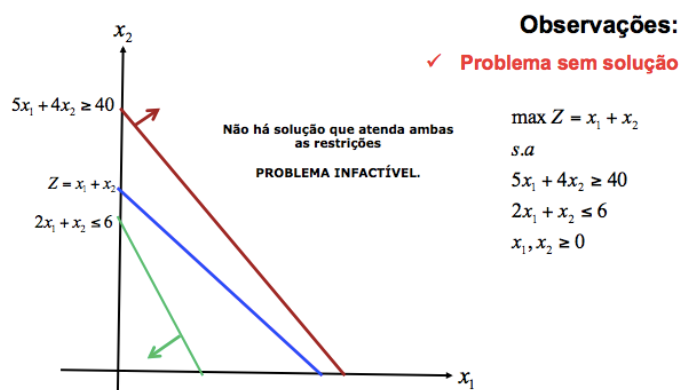
\includegraphics[width=5cm,height=4cm]{prob_semsol.png}
		\end{column}
		\begin{column}{5cm}
			\centering
			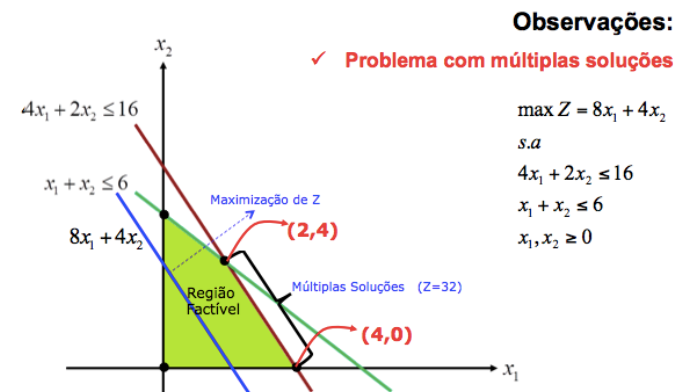
\includegraphics[width=4cm,height=4cm]{prob_multsol.png}
		\end{column}
	\end{columns}
	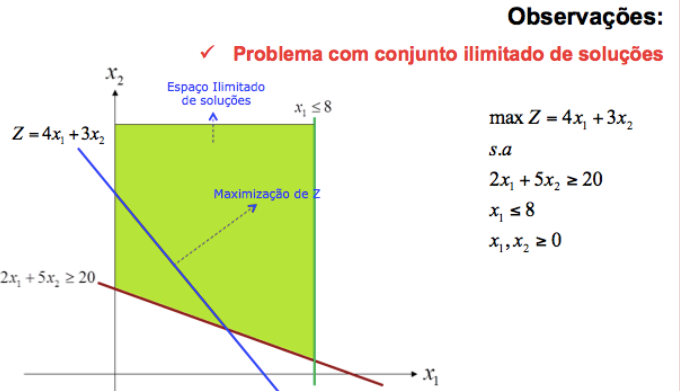
\includegraphics[width=5cm,height=4cm]{prob_ilimitado.png}
\end{frame}

\subsection{Problema com Múltiplas Soluções} 
\begin{frame}
	\frametitle{Caso Especial: Múltipla Solução}
	\begin{block}{Como identificar esta situação no Tableau Simplex?}
			Quando, {\color{red}\underline{na forma tableau ótima}}, o coeficiente de uma das variáveis não-básicas (VNB) for nulo na linha referente a expressão da FOB. 
	\end{block} \pause
	\underline{Exemplo}:
	\begin{columns}
		\begin{column}{4cm}
			\begin{mdframed}[backgroundcolor=black!10]
				$	\begin{matrix}
						\max z = 8x_1 + 4x_2 \\
						Sujeito a: \\
						4x_1 + 2x_2 \le 16 \\
						x_1 + x_2 \le 16 \\
						x_1, x_2 \ge 0 \\
					\end{matrix}
				$
			\end{mdframed}
		\end{column} \pause
		\begin{column}{6.5cm}
			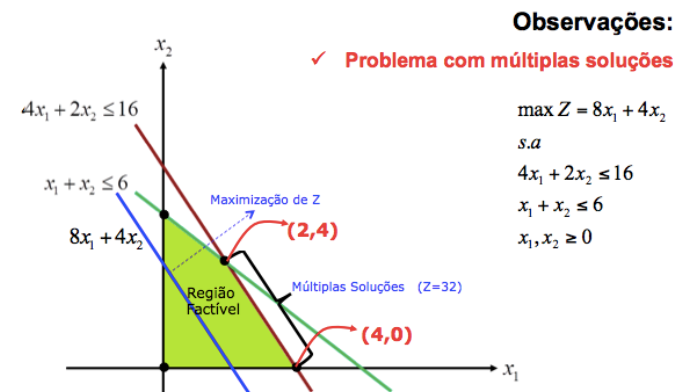
\includegraphics[width=7cm,height=5cm]{prob_multsol.png}
		\end{column}
	\end{columns}
	
\end{frame}



\begin{frame}
	\frametitle{Caso Especial: Múltipla Solução}

	\begin{itemize}
		\item {Tableau ótimo em um problema de Maximização. Convergência $\Leftrightarrow$ Coef. das VNBs $\ge$ 0.}
			\only<1>
			{
			\begin{table}
				\scriptsize
				\newcommand{\azbr}{\cellcolor{blue!70} \color{white}}
				\newcommand{\azvm}{\cellcolor{blue!70} \color{red}}
				\newcommand{\ampr}{\cellcolor{yellow!70} \color{black}}
				\newcommand{\amvm}{\cellcolor{yellow!70} \color{red}}
				\begin{tabular}{ c  c  c  c  c  c  c  c }
				\azbr Variável & \azbr $N^o$ da & \multicolumn{5}{c}{\azbr Coeficientes} & \multirow{2}{1.5cm}{\azbr  Constantes} \\[3pt]
				\azbr Básica   & \azbr Equação  & \azbr $z$ &\azvm  $x_1$ & \azbr $x_2$ & \azbr $x_3$ & \azvm $x_4$ &  \azbr                               \\[3pt]
				\amvm $x_1$ & \ampr 1 & \ampr 0 & \ampr 1 & \ampr $\frac{1}{2}$ & \ampr $\frac{1}{4}$  &  \ampr 0 & \ampr 4  \\ [3pt]
				\amvm $x_4$ & \ampr 2 & \ampr 0 & \ampr 0 & \ampr $\frac{1}{2}$ & \ampr -$\frac{1}{4}$ &  \ampr 1 & \ampr 2  \\	[3pt]
				\ampr $z$   & \ampr 3 & \ampr 1 & \ampr 0 & \ampr 0  			& \ampr 2 			   &  \ampr 0 & \ampr 32 \\	[3pt]
				\end{tabular}
			\end{table}
			}
			\only<2->
			{
			\begin{table}
				\scriptsize
				\newcommand{\azbr}{\cellcolor{blue!70} \color{white}}
				\newcommand{\azvm}{\cellcolor{blue!70} \color{red}}
				\newcommand{\ampr}{\cellcolor{yellow!70} \color{black}}
				\newcommand{\amvm}{\cellcolor{yellow!70} \color{red}}
				\newcommand{\vevm}{\cellcolor{green!70} \color{red}}
				\begin{tabular}{ c  c  c  c  c  c  c  c }
				\azbr Variável & \azbr $N^o$ da & \multicolumn{5}{c}{\azbr Coeficientes} & \multirow{2}{1.5cm}{\azbr  Constantes} \\[3pt]
				\azbr Básica   & \azbr Equação  & \azbr $z$ &\azvm  $x_1$ & \azbr $x_2$ & \azbr $x_3$ & \azvm $x_4$ &  \azbr                               \\[3pt]
				\amvm $x_1$ & \ampr 1 & \ampr 0 & \ampr 1 & \ampr $\frac{1}{2}$ & \ampr $\frac{1}{4}$  &  \ampr 0 & \ampr 4  \\ [3pt]
				\amvm $x_4$ & \ampr 2 & \ampr 0 & \ampr 0 & \ampr $\frac{1}{2}$ & \ampr -$\frac{1}{4}$ &  \ampr 1 & \ampr 2  \\	[3pt]
				\ampr $z$   & \ampr 3 & \ampr 1 & \ampr 0 & \vevm 0  			& \vevm 2 			   &  \ampr 0 & \ampr 32 \\	[3pt]
				\end{tabular}
			\end{table}
			}
			\only<3->
			{
			{\color{black} \scriptsize Como $x_2$ (VNB) tem coeficiente igual a zero, sua entrada não altera o valor de Z (FOB). }
			}
		\only<4->
		{
		\item  {\color{black} Sai $x_4$ e entra $x_2$}
			\only<5->
			{
				\begin{table}
					\scriptsize
					\newcommand{\azbr}{\cellcolor{blue!70} \color{white}}
					\newcommand{\azvm}{\cellcolor{blue!70} \color{red}}
					\newcommand{\ampr}{\cellcolor{yellow!70} \color{black}}
					\newcommand{\amvm}{\cellcolor{yellow!70} \color{red}}
					\newcommand{\vevm}{\cellcolor{green!70} \color{red}}
					\begin{tabular}{ c  c  c  c  c  c  c  c }
					\azbr Variável & \azbr $N^o$ da & \multicolumn{5}{c}{\azbr Coeficientes} & \multirow{2}{1.5cm}{\azbr  Constantes} \\[3pt]
					\azbr Básica   & \azbr Equação  & \azbr $z$ &\azvm  $x_1$ & \azvm $x_2$ & \azbr $x_3$ & \azbr $x_4$ &  \azbr                               \\[3pt]
					\amvm $x_1$ & \ampr 1 & \ampr 0 & \ampr 1 & \ampr 0 & \ampr $\frac{1}{2}$  & \ampr -1 & \ampr 2  \\ [3pt]
					\amvm $x_2$ & \ampr 2 & \ampr 0 & \ampr 0 & \ampr 1 & \ampr -$\frac{1}{2}$ & \ampr 2  & \ampr 4  \\ [3pt]
					\ampr $z$   & \ampr 3 & \ampr 1 & \ampr 0 & \ampr 0 & \vevm 2  			   & \vevm 0  & \ampr 32 \\ [3pt]
					\end{tabular}
				\end{table}
			}
			\only<6->
			{
			{\color{black} \scriptsize Com a entrada $x_2$ na base o valor de Z (FOB) não se altera. }
			}
		}
	\end{itemize}

\end{frame}

\subsection{Problema Ilimitado}

\begin{frame}
	\frametitle{Caso Especial: Conjunto Ilimitado de Soluções (unbounded)}
	\begin{block}{Como identificar esta situação no Tableau Simplex?}
		Quando, {\color{red} \underline{na forma tableau simplex (em qualquer iteração)}}, não há a possibilidade de retirar nenhuma VB devido aos coeficientes negativos ou nulos na coluna referente a VNB que entratá na base.
	\end{block}
	\underline{Exemplo}:
	\begin{columns}
		\begin{column}{4cm}
			\begin{mdframed}[backgroundcolor=black!10]
				$	\begin{matrix}
						\max z = 4x_1 + 3x_2\\
						\text{Sujeito a:} \\
						2x_1 + 5x_2 \ge 20 \\
						x_1 \le 8 \\
						x_1, x_2 \ge 0 \\
					\end{matrix}
				$
			\end{mdframed}
		\end{column} \pause
		\begin{column}{6.5cm}
			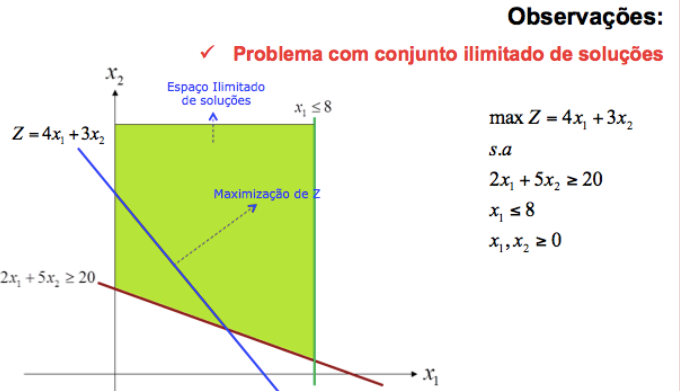
\includegraphics[width=7cm,height=5cm]{prob_ilimitado.png}
		\end{column}
	\end{columns}
\end{frame}

\begin{frame}
	\frametitle{Caso Especial: Conjunto Ilimitado de Soluções (unbounded)}

	\begin{itemize}
		\item {Tableau $2^a$ Iteração, problema de Maximização. Convergência $\Leftrightarrow$ Coef. das VNBs $\ge$ 0.}
			\only<1>
			{
			\begin{table}
				\scriptsize
				\newcommand{\azbr}{\cellcolor{blue!70} \color{white}}
				\newcommand{\azvm}{\cellcolor{blue!70} \color{red}}
				\newcommand{\ampr}{\cellcolor{yellow!70} \color{black}}
				\newcommand{\amvm}{\cellcolor{yellow!70} \color{red}}
				\begin{tabular}{ c  c  c  c  c  c  c  c }
				\azbr Variável & \azbr $N^o$ da & \multicolumn{5}{c}{\azbr Coeficientes} & \multirow{2}{1.5cm}{\azbr  Constantes} \\[3pt]
				\azbr Básica   & \azbr Equação  & \azbr $w$ & \azbr  $x_1$ & \azvm $x_2$ & \azbr $x_3$           & \azvm $x_4$          & \azbr      		  \\[3pt]
				\amvm $x_2$    & \ampr 1        & \ampr 0   & \ampr 0      & \ampr 1     & \ampr -$\frac{1}{5}$  & \ampr -$\frac{2}{5}$ & \ampr $\frac{4}{5}$ \\[3pt]
				\amvm $x_4$    & \ampr 2        & \ampr 0   & \ampr 1      & \ampr 0     & \ampr 0               & \ampr 1              & \ampr 8  			  \\[3pt]
				\ampr $w$      & \ampr 3        & \ampr 1   & \ampr 0      & \ampr 0     & \ampr -$\frac{3}{5}$  & \ampr $\frac{14}{5}$ & \ampr $\frac{172}{5}$\\[3pt]
				\end{tabular}
			\end{table}
			}
			\only<2->
			{
			\begin{table}
				\scriptsize
				\newcommand{\azbr}{\cellcolor{blue!70} \color{white}}
				\newcommand{\azvm}{\cellcolor{blue!70} \color{red}}
				\newcommand{\ampr}{\cellcolor{yellow!70} \color{black}}
				\newcommand{\amvm}{\cellcolor{yellow!70} \color{red}}
				\newcommand{\prpr}{\cellcolor{black!40} \color{black}}
				\begin{tabular}{ c  c  c  c  c  c  c  c c }
				\azbr Variável & \azbr $N^o$ da & \multicolumn{5}{c}{\azbr Coeficientes} & \multirow{2}{1.5cm}{\azbr  Constantes} \\[3pt]
				\azbr Básica   & \azbr Equação  & \azbr $w$ & \azbr  $x_1$ & \azvm $x_2$ & \azbr $x_3$           & \azvm $x_4$          & \azbr      		     \\[3pt]
				\amvm $x_2$    & \ampr 1        & \ampr 0   & \ampr 0      & \ampr 1     & \prpr -$\frac{1}{5}$  & \ampr -$\frac{2}{5}$ & \prpr $\frac{4}{5}$  & \color{black} $=-4$ \\[3pt]
				\amvm $x_4$    & \ampr 2        & \ampr 0   & \ampr 1      & \ampr 0     & \prpr 0               & \ampr 1              & \prpr 8  			   & \color{black} $=\infty$\\[3pt]
				\ampr $w$      & \ampr 3        & \ampr 1   & \ampr 0      & \ampr 0     & \prpr -$\frac{3}{5}$  & \ampr $\frac{14}{5}$ & \prpr $\frac{172}{5}$  \\[3pt]
				\end{tabular}
			\end{table}
			}			
			\only<3->
			{
			{\color{black} \scriptsize $x_3$ deve entrar na base - maior coeficiente negativo em w (FOB). Entretanto, todos os elementos de sua coluna são negativos ou nulos, não há como uma variável básica ($x_2$ ou $x_4$) sair da base. }
			}
	\end{itemize}
	\only<4->
	{
		\begin{mdframed}[backgroundcolor=red!40]
			\centering
			Valor da Função Objetivo Ilimitado!
		\end{mdframed}
	}
\end{frame}


\subsection{Problema Sem Solução}
\begin{frame}
	\frametitle{Caso Especial: Problema Sem Solução Ótima}
	\begin{block}{Como identificar esta situação no Tableau Simplex?}
		Quando, {\color{red} \underline{na forma tableau ótimo}}, a solução final tiver pelo menos uma variável artificial com valor não nulo na base. 	
	\end{block}
	\underline{Exemplo}:
	\begin{columns}
		\begin{column}{4cm}
			\begin{mdframed}[backgroundcolor=black!10]
				$	\begin{matrix}
						\max z = x_1 + x_2\\
						\text{Sujeito a:} \\
						5x_1 + 4x_2 \ge 40 \\
						2x_1 + x_2 \le 6 \\
						x_1, x_2 \ge 0 \\
					\end{matrix}
				$
			\end{mdframed}
		\end{column} \pause
		\begin{column}{6.5cm}
			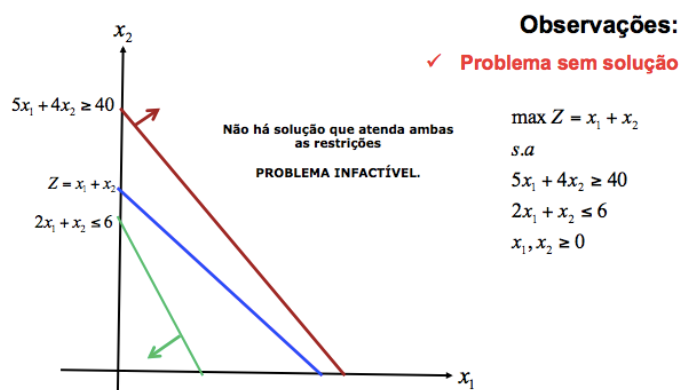
\includegraphics[width=7cm,height=5cm]{prob_semsol.png}
		\end{column}
	\end{columns}
\end{frame}

\begin{frame}
	\frametitle{Caso Especial: Problema Sem Solução Ótima}
	\begin{columns}
		\centering
		\begin{column}{5cm}
			\begin{mdframed}[backgroundcolor=black!20]
				\centering
				\scriptsize
				$	\begin{matrix}
						\max z = x_1 + x_2\\
						\text{Sujeito a:} \\
						5x_1 + 4x_2 \ge 40 \\
						2x_1 + x_2 \le 6 \\
						x_1, x_2 \ge 0 \\
					\end{matrix}
				$			
			\end{mdframed}
		\end{column}
		\begin{column}{5cm}
			\begin{mdframed}[backgroundcolor=yellow!70]
				\centering
				\scriptsize
				$	\begin{matrix}
						\max z = x_1 + x_2 {\color{red}+Ma_1}\\
						\text{Sujeito a:} \\
						5x_1 + 4x_2 {\color{red} - x_3 + a_1 =} 40 \\
						2x_1 + x_2 {\color{red} + x_4 =} 6 \\
						x_1, x_2{\color{red} ,x_3,x_4,a_1} \ge 0 \\
					\end{matrix}
				$			
			\end{mdframed}
		\end{column}
	\end{columns}
	\begin{itemize}
		\item {Tableau ótimo no prob. Maxim. Convergência $\Leftrightarrow$ Coef. das VNBs $\ge$ 0.}
		\begin{table}
			\scriptsize
			\newcommand{\azbr}{\cellcolor{blue!70} \color{white}}
			\newcommand{\azvm}{\cellcolor{blue!70} \color{red}}
			\newcommand{\ampr}{\cellcolor{yellow!70} \color{black}}
			\newcommand{\amvm}{\cellcolor{yellow!70} \color{red}}
			\begin{tabular}{ c  c  c  c  c  c  c  c c }
			\azbr Variável & \azbr $N^o$ da & \multicolumn{6}{c}{\azbr Coeficientes} & \multirow{2}{1.5cm}{\azbr  Constantes} \\[3pt]
			\azbr Básica   & \azbr Equação  & \azbr $w$ & \azbr  $x_1$ & \azvm $x_2$ & \azbr $x_3$ & \azbr $x_4$ & \azvm $a_1$ & \azbr          \\[3pt]
			\amvm $a_1$    & \ampr 1        & \ampr 0   & \ampr -3     & \ampr 0     & \ampr -1    & \ampr -4    & \ampr1	   & \ampr 16 	    \\[3pt]
			\amvm $x_2$    & \ampr 2        & \ampr 0   & \ampr 2      & \ampr 1     & \ampr 0     & \ampr 1     & \ampr0	   & \ampr 6  	    \\[3pt]
			\ampr $w$      & \ampr 3        & \ampr 1   & \ampr $3M+1$ & \ampr 0     & \ampr -$M$  & \ampr $M+1$ & \ampr0	   & \ampr $-16M+6$ \\[3pt]
			\end{tabular}
		\end{table}	
		\item \color{black} Observe que $a_1$ possui valor não nulo ($=16$). Ou seja, a solução final encontrada não é ótima, uma vez que a solução encontrada não corresponde à formulação original (FOB Original. 	
	\end{itemize}
\end{frame}

\subsection{Empate na Escolha (entrar ou sair da base)}
\begin{frame}
	\frametitle{Empate na Escolha da Variável para \underline{Entrar} ou \underline{Sair} da base}
	\only<1>
	{
		\begin{table}
			\begin{tabular}{c c c}
				
\includegraphics[width=0.6cm,height=0.3cm]{seta.png} & \text{Empate para entrar na base} & \multirow{2}{1cm}{
\includegraphics[width=1.5cm,height=1.5cm]{There-are-no-rules.jpg}} \\ [12pt] 
				
\includegraphics[width=0.6cm,height=0.3cm]{seta.png} & \text{Empate para sair da Base} \\[12pt]				
			\end{tabular}
		\end{table}
	}
	\only<2->
	{
		\begin{table}
			\begin{tabular}{c c c}
				
\includegraphics[width=0.6cm,height=0.3cm]{seta.png} & \text{Empate para entrar na base} & \multirow{2}{1cm}{
\includegraphics[width=3cm,height=1.5cm]{proibido.jpg}}\\[12pt]
				
\includegraphics[width=0.6cm,height=0.3cm]{seta.png} & \text{Empate para sair da Base} \\[12pt]				
			\end{tabular}
		\end{table}
	}
	\only<3->
	{
		\begin{mdframed}[backgroundcolor=red!60]
			\centering
			\underline{Conseqüência}: $\pm$ iterações dependendo da escolha.
		\end{mdframed}
	}
\end{frame}


\begin{frame}
\Huge{\centerline{Fim}}
\end{frame}

%----------------------------------------------------------------------------------------

\end{document} 